\chapter*{Progettazione}
\addcontentsline{toc}{chapter}{Progettazione}
\phantomsection
\section*{Progettazione architetturale}
\addcontentsline{toc}{section}{Progettazione architetturale}
\vspace{0.5cm}

\phantomsection
\subsection*{Requisiti non Funzionali}
\addcontentsline{toc}{subsection}{Requisiti non Funzionali}
\vspace{0.5cm}
Nell' Analisi del problema sono emersi dei requisiti non funzionali che impongono i seguenti vincoli:

\begin{enumerate}
\item Interfaccia utente intuitiva.
\item Velocità nel caricare/scaricare file.
\item Organizzazione del file manager ampiamente personalizzabile.
\item Possibilità di cambiare la view in modo rapido.
\item Utilizzo efficace del servizio anche in assenza di una connessione veloce.
\item Pannello di amministrazione intuitivo
\end{enumerate}

\\
L'interfaccia utente deve permettere di far capire immediatamente all'utente le funzionalità disponibili per caricare e scaricare file, inoltre deve essere fornito un sistema facile e veloce per modificare le varie viste. L'utilizzo veloce è garantito anche in assenza di una connessione veloce, perché le operazioni sulle viste verranno svolte principalmente lato client.\\
Il pannello di amministrazione intuitivo permetterà all'amministratore di operare velocemente nel sistema, agendo tempestivamente sugli utenti che svolgono azioni indesiderate.


\phantomsection
\subsection*{Scelta dell' Architettura}
\addcontentsline{toc}{subsection}{Scelta dell' Architettura}
Per l'architettura del sistema si è optato per un sistema Client/Server che si appoggia ad un Database. Le connessioni tra i vari livelli saranno cifrate.
\vspace{0.5cm}
\phantomsection
\subsection*{L1 - Client}
\addcontentsline{toc}{subsection}{L1 - Client}
Il Client utilizzerà una connessione TLS che sarà fondamentale in tutte le operazioni di interazione con il server e per lo scambio dei file che avverrà tra i due.
Per aggiungere un ulteriore livello di sicurezza, negli sviluppi futuri dell' applicazione si potrebbe aggiungere una cifratura dei file lato server.
\\
Il Client Utente sarà potenzialmente anche Client AmministratoreGruppo e sarà poi presente un Client Amministratore separato.
\vspace{0.5cm}

\phantomsection
\subsection*{L2 - Server}
\addcontentsline{toc}{subsection}{L2 - Server}
\vspace{0.5cm}
Sul sistema sarà presente
\begin{itemize}
\item Un Server per la gestione degli Utenti
\item Un Server per la gestione dei Gruppi
\item Un Server per la gestione degli Amministratori
\item Un Server per la gestione dei File
\end{itemize}
\phantomsection
\subsection*{L3 - Database}
\addcontentsline{toc}{subsection}{L3 - Database}
Per la gestione della persistenza dei dati degli Utenti e dell' Amministratore e per salvare gli ID dei file, viene utilizzata una connessione sicura TLS già supportata dal database e in più verrà aggiunto un SALT che garantirà una maggiore sicurezza nel caso di attacchi a dizionario.
Il Database - Server sarà installabile in modo disaccoppiato al sistema, in modo da poter utilizzare anche eventualmente un sistema Cloud o un sistema esterno per salvare i dati.
\\
Il database sarà disposto su tre server: un database memorizzerà i dati degli utilizzatori del sistema, un altro database memorizzerà i LOG e sarà accessibile dall'Amministratore per il monitoraggio del sistema e l'ultimo database manterrà la struttura ad albero dei file con i relativi ID.
Questo disaccoppiamento è utile per non avere un "Single Point of Failure" che può avvenire tramite un guasto all'unico sistema di persistenza, ad esempio non sarebbe tollerabile un disservizio al database degli utenti causato da un malfunzionamento del database dei LOG.
\\
L'interfacciamento fra l'applicativo e i DBMS avverrà secondo la metodologia \verb|forza bruta|, utilizzando dei metodi CRUD.

\vspace{0.5cm}

\phantomsection
\subsection*{Scelte Tecnologiche}
\addcontentsline{toc}{subsection}{Scelte Tecnologiche}

L'applicazione viene sviluppata come applicazione web, in modo da essere accessibile da molti dispositivi che supportano le tecnologie web moderne e abbiano a disposizione un web browser.
\\
Per l'installazione può essere utilizzato un metodo "a container" che faciliterà il deploy, oltre che a rendere più chiusa l'applicazione verso il sistema principale.

\vspace{0.5cm}

\pagebreak
\phantomsection
\subsection*{Diagramma dei package}
\addcontentsline{toc}{subsection}{Diagramma dei package}
Di seguito è riportata l’Architettura del Sistema organizzata attraverso un diagramma dei package.
\vspace{2cm}

\begin{adjustwidth}{-3cm}{0cm}
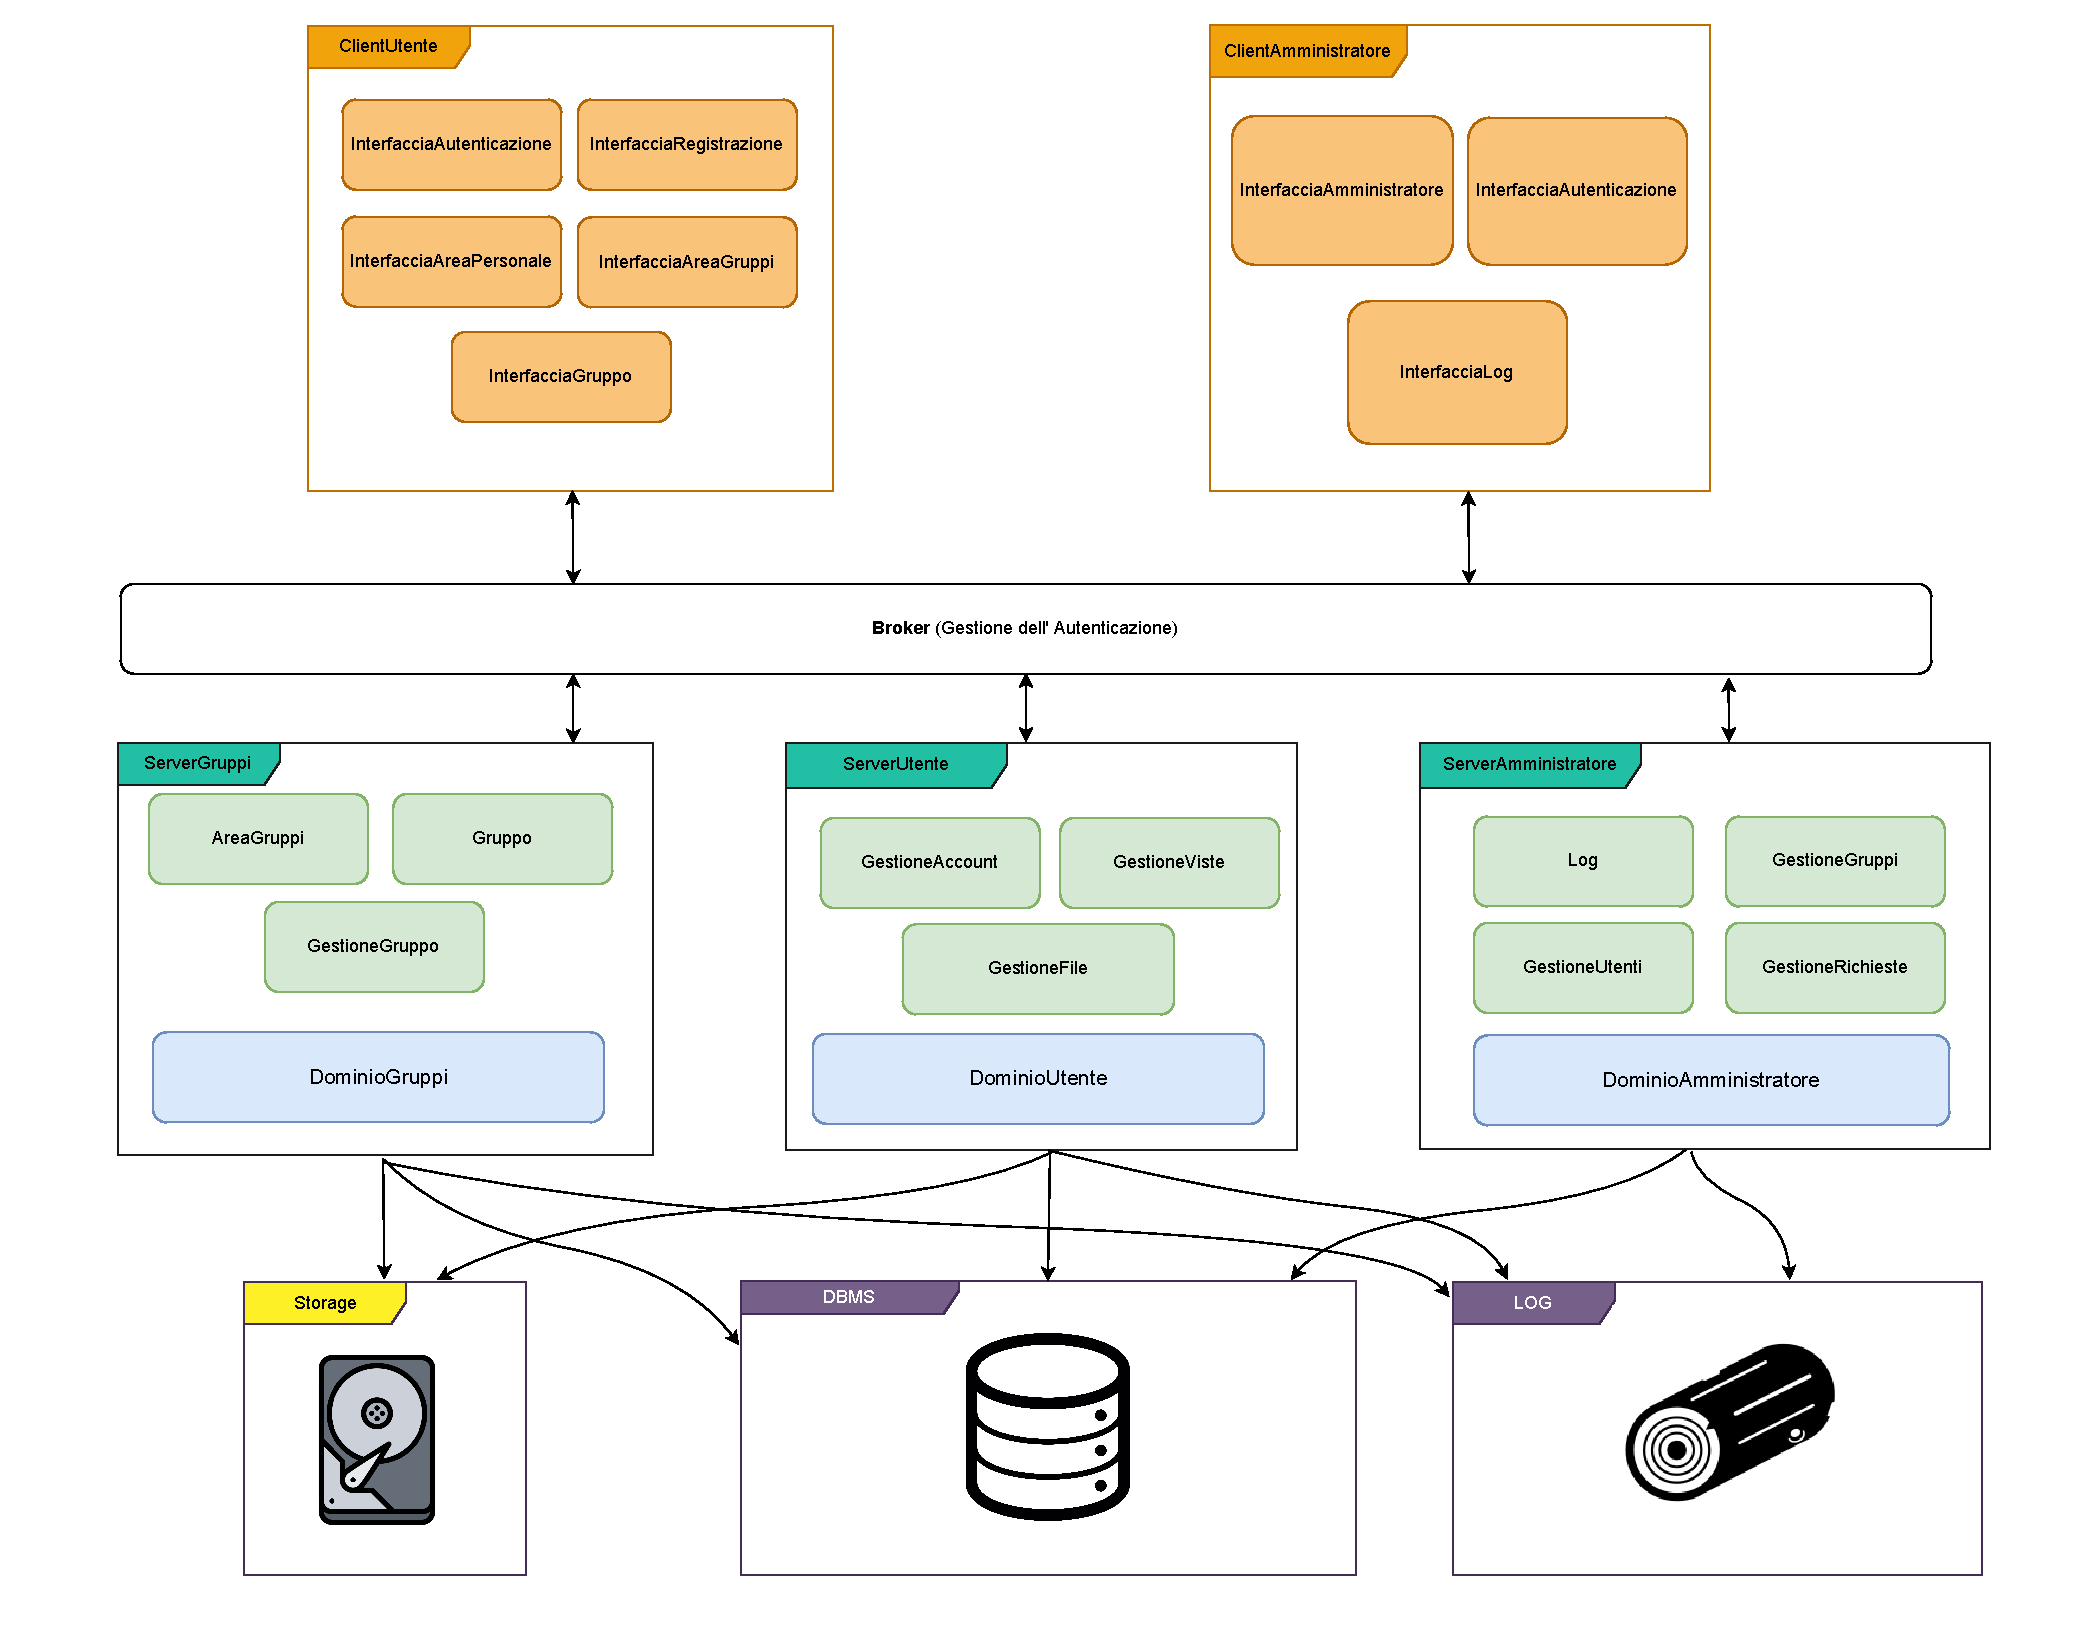
\includegraphics[scale=0.55]{progettazione/Progettazione-Diagramma Package.drawio.pdf}
\end{adjustwidth}


\pagebreak
\phantomsection
\subsection*{Diagramma dei componenti}
\addcontentsline{toc}{subsection}{Diagramma dei componenti}
Di seguito è riportato il diagramma dei componenti di sistema.
\vspace{2cm}
\begin{adjustwidth}{1cm}{0cm}
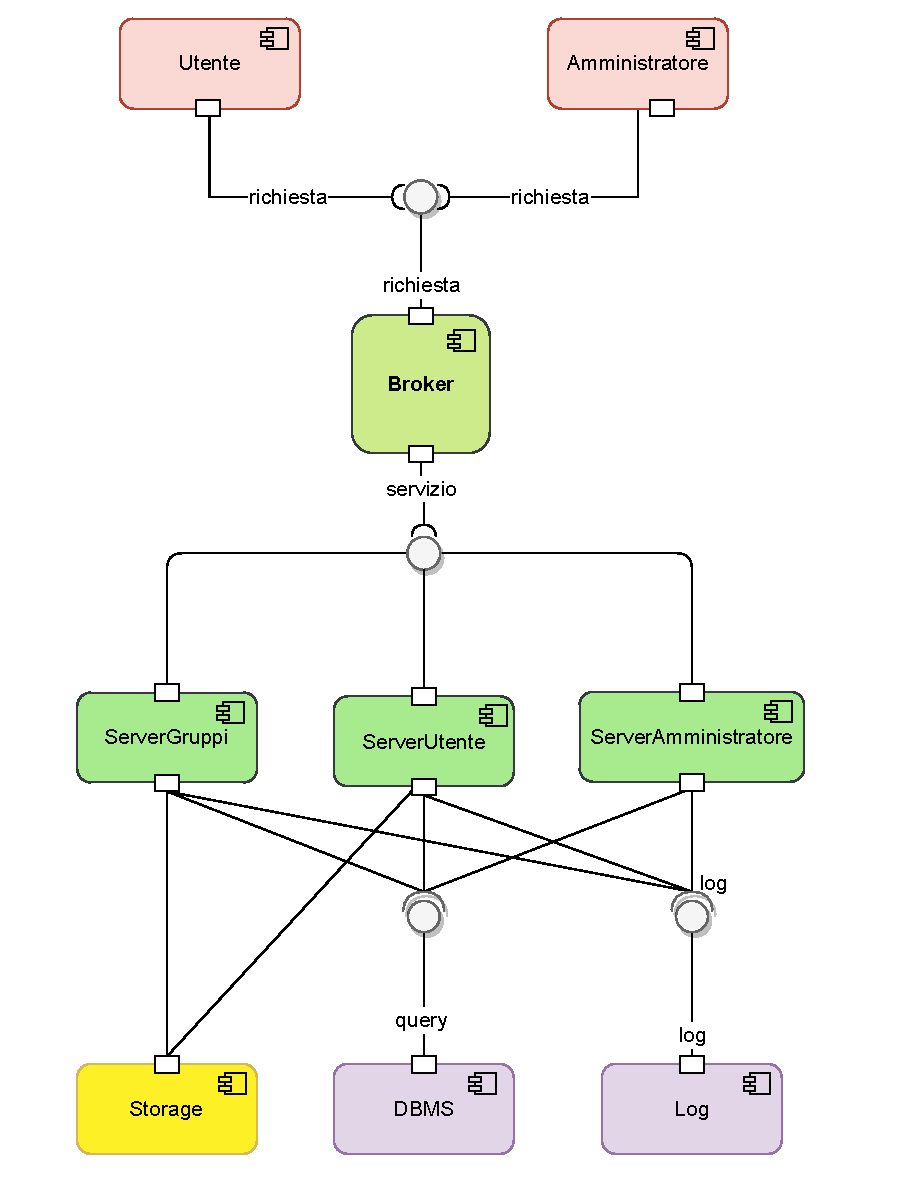
\includegraphics[scale=0.9]{progettazione/Progettazione-Diagramma Componenti.drawio.pdf}
\end{adjustwidth}
\vspace{1cm}


\pagebreak
\phantomsection
\section*{Progettazione di dettaglio}
\addcontentsline{toc}{section}{Progettazione di dettaglio}
\vspace{1cm}

\subsection*{Dominio: Struttura Account}
\phantomsection
\addcontentsline{toc}{subsection}{Dominio: Struttura Account}
\vspace{0.5cm}
\begin{adjustwidth}{-2cm}{0cm}
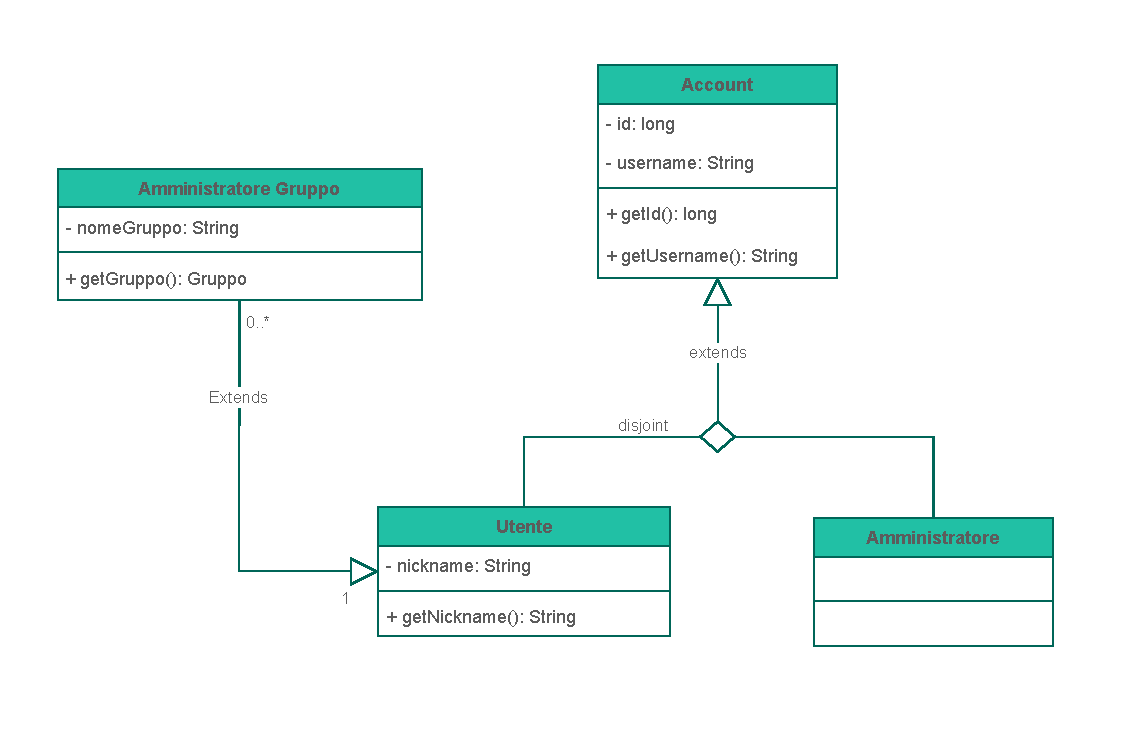
\includegraphics[scale=0.9]{progettazione/Progettazione-Struttura Account.drawio.pdf}
\end{adjustwidth}
\vspace{1cm}

\subsection*{Dominio: Amministrazione}
\phantomsection
\addcontentsline{toc}{subsection}{Dominio: Amministrazione}
\vspace{0.5cm}
\begin{adjustwidth}{-3.5cm}{0cm}
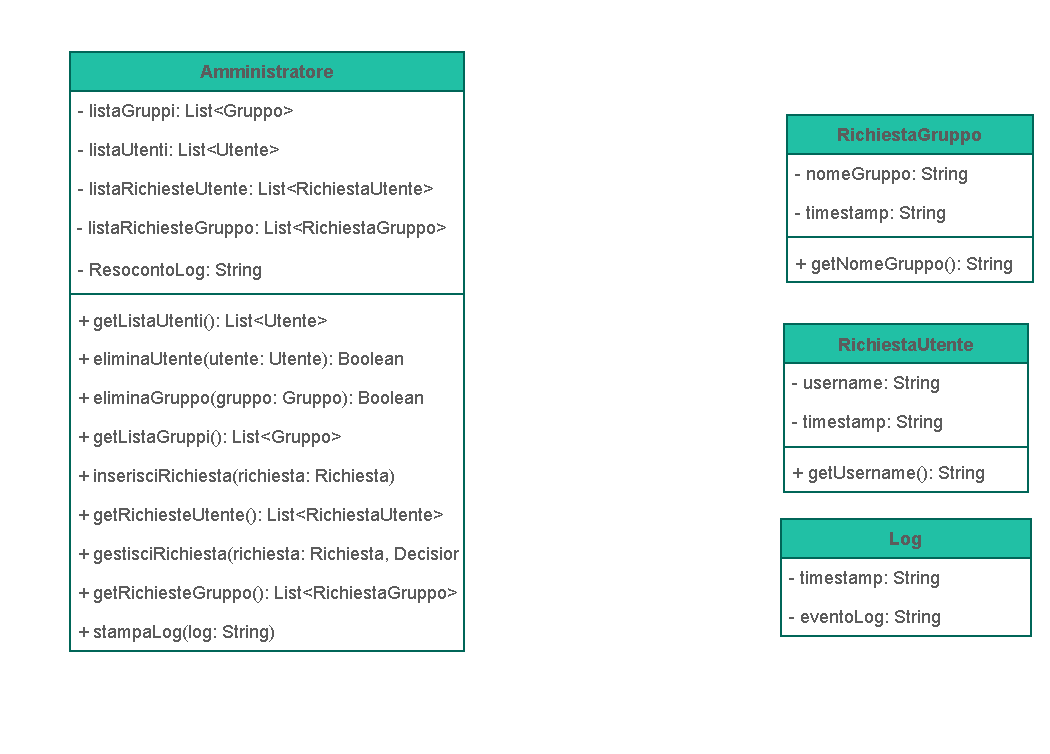
\includegraphics[scale=0.9]{progettazione/Progettazione-Amministrazione.drawio.pdf}
\end{adjustwidth}
\vspace{1cm}

\subsection*{Dominio: Area Personale}
\phantomsection
\addcontentsline{toc}{subsection}{Dominio: Area Personale}
\vspace{0.5cm}
\begin{adjustwidth}{-2cm}{0cm}
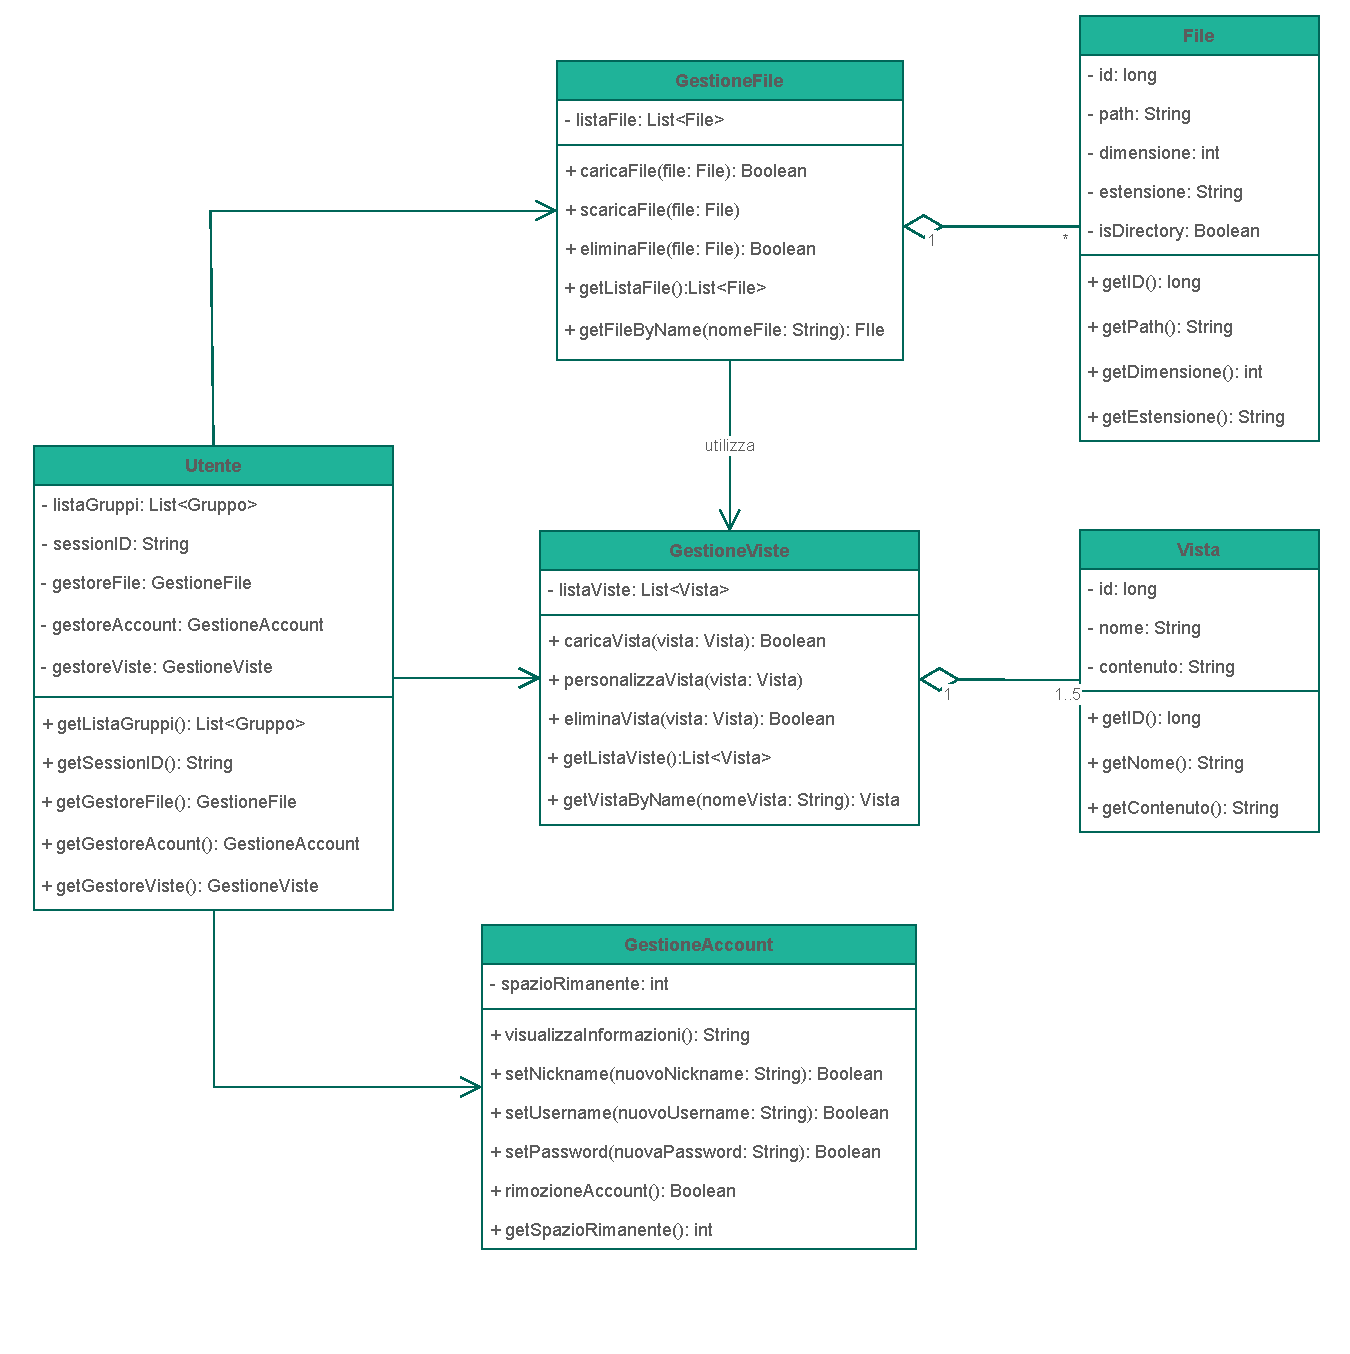
\includegraphics[scale=0.8]{progettazione/Progettazione-Area Personale.drawio.pdf}
\end{adjustwidth}
\vspace{1cm}
È stato deciso di creare una classe per i File, con un'istanza della classe per ogni File caricato dall'Utente.\\
Questo può essere oneroso per il Server in quanto occupa più memoria, però garantisce una migliore esperienza per l'Utente dato che l'accesso più facile all'alberatura dei file consente una navigazione più immediata.\\

\subsection*{Dominio: Area Gruppi}
\phantomsection
\addcontentsline{toc}{subsection}{Dominio: Area Gruppi}
\vspace{0.5cm}
\begin{adjustwidth}{-2cm}{0cm}
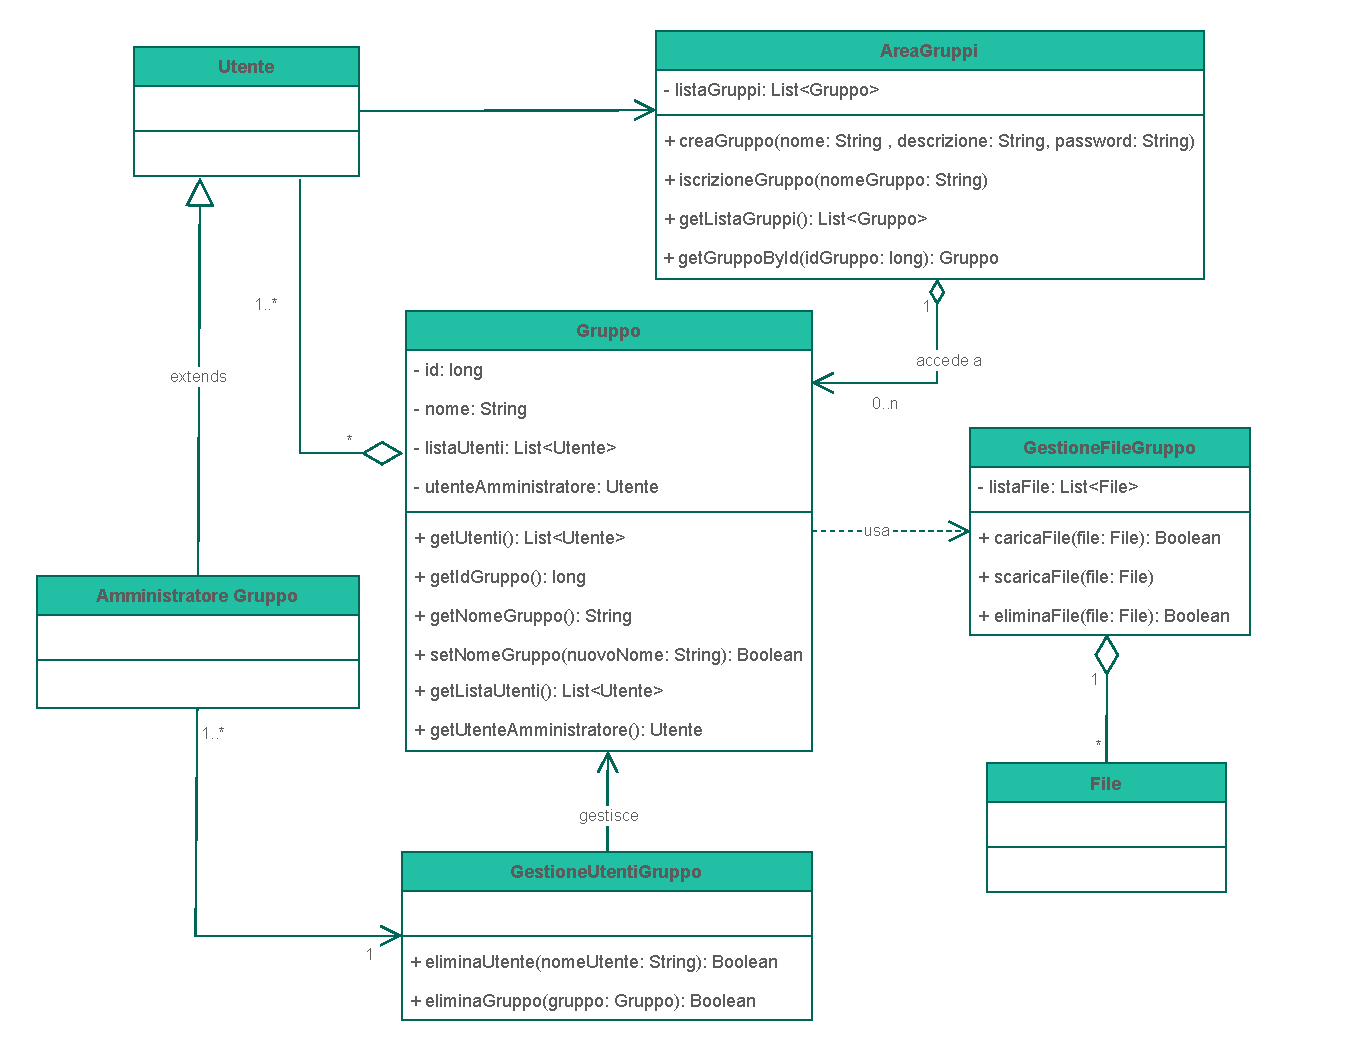
\includegraphics[scale=0.8]{progettazione/Progettazione-Area Gruppi.drawio.pdf}
\end{adjustwidth}
\vspace{1cm}


\subsection*{Diagramma di Dettaglio - Interfacce}
\phantomsection
\addcontentsline{toc}{subsection}{Interfacce}
\vspace{0.5cm}
\begin{adjustwidth}{-2.5cm}{0cm}
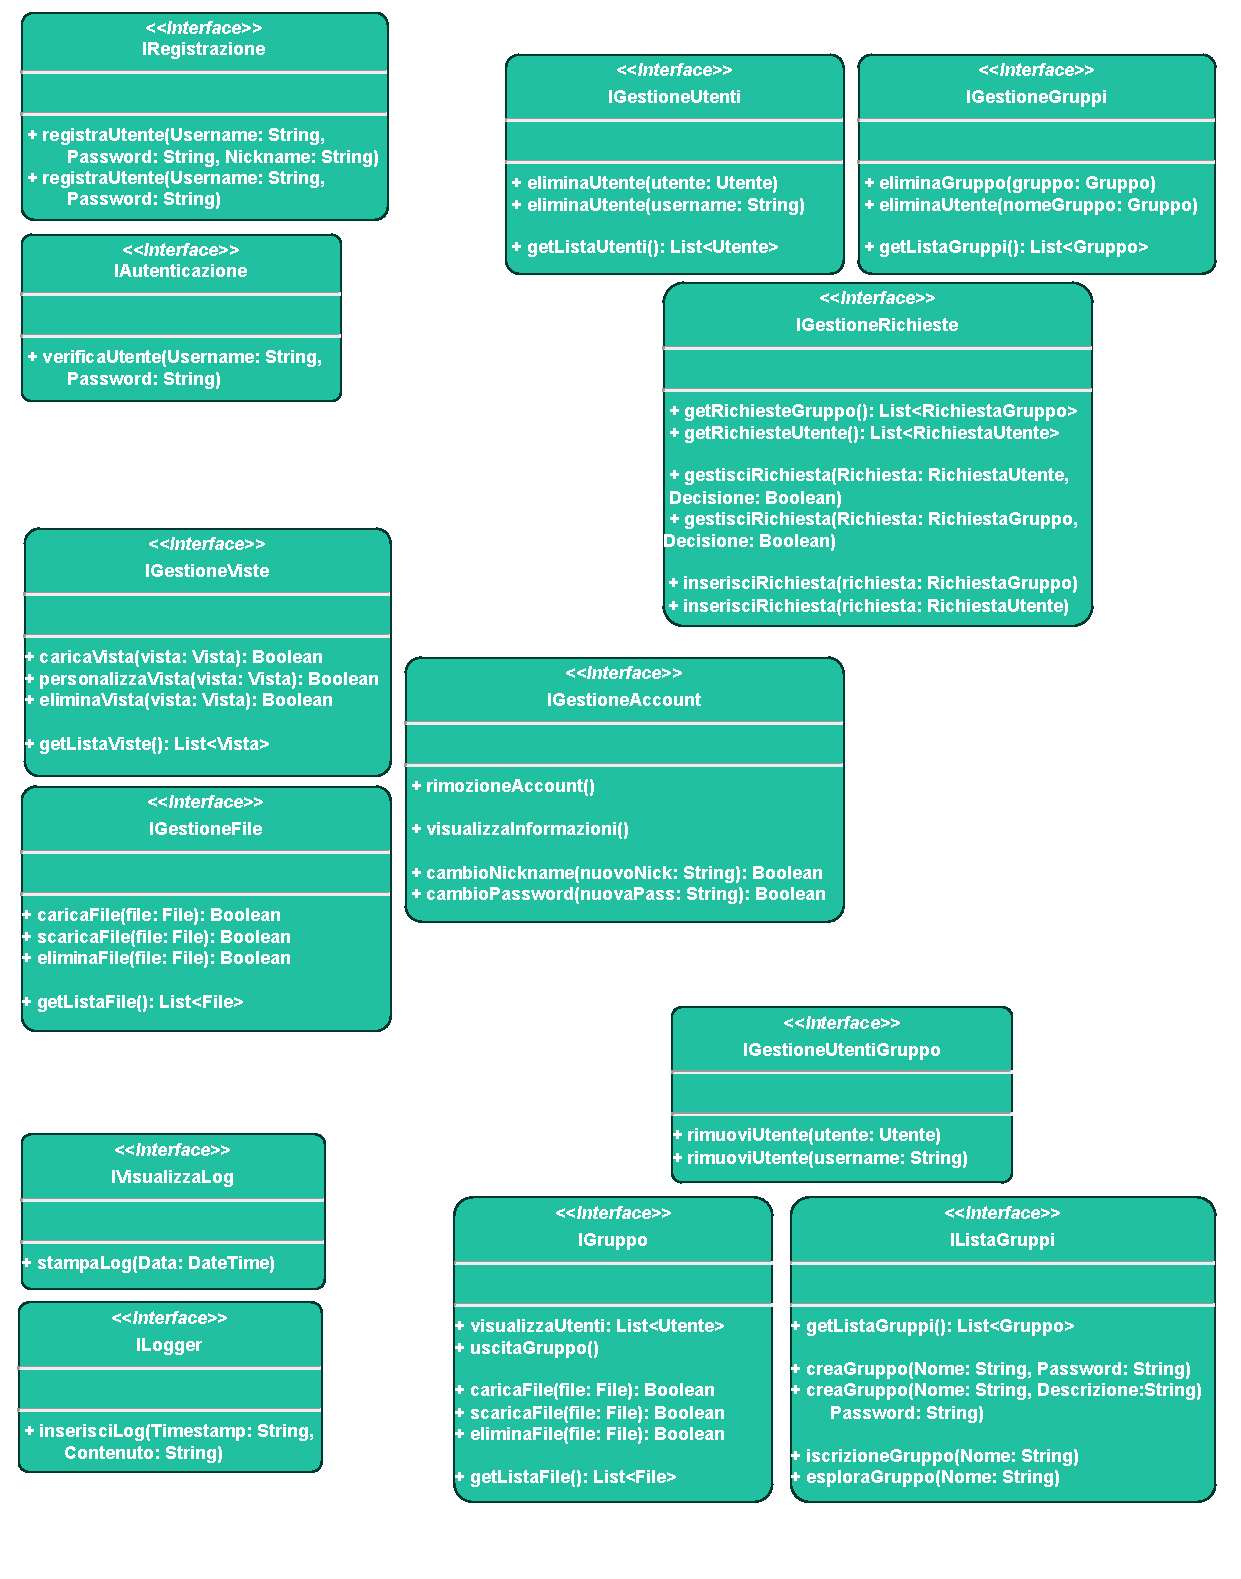
\includegraphics[scale=0.9]{progettazione/Progettazione-Interfacce.drawio.pdf}
\end{adjustwidth}
\vspace{1cm}


\subsection*{Diagramma di Dettaglio: Registrazione e Autenticazione}
\phantomsection
\addcontentsline{toc}{subsection}{Registrazione e Autenticazione}
\begin{adjustwidth}{-2cm}{0cm}
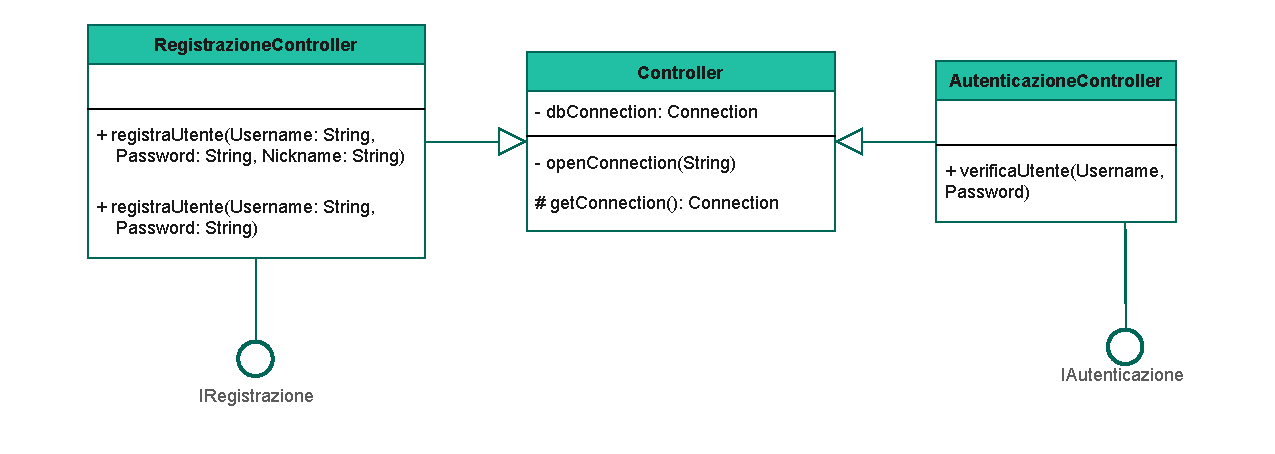
\includegraphics[scale=0.9]{progettazione/Progettazione-Dettaglio Autenticazione.drawio.pdf}
\end{adjustwidth}
\vspace{2cm}

\subsection*{Diagramma di Dettaglio: Amministrazione}
\phantomsection
\addcontentsline{toc}{subsection}{Amministrazione}
\begin{adjustwidth}{-3cm}{0cm}
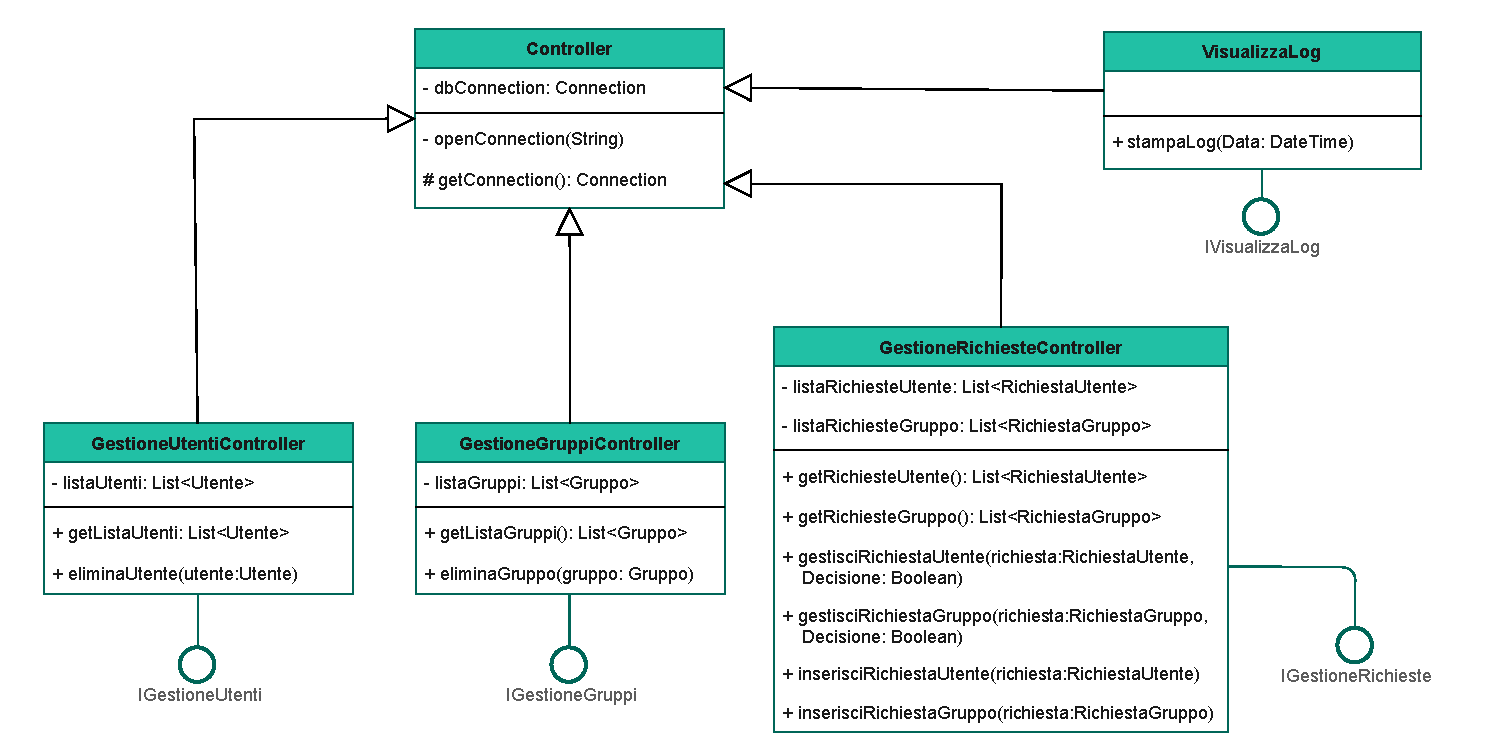
\includegraphics[scale=0.8]{progettazione/Progettazione-Dettaglio Amministratore.drawio.pdf}
\end{adjustwidth}
\vspace{0.5cm}


\subsection*{Diagramma di Dettaglio: Log}
\phantomsection
\addcontentsline{toc}{subsection}{Log}
\begin{adjustwidth}{-2cm}{0cm}
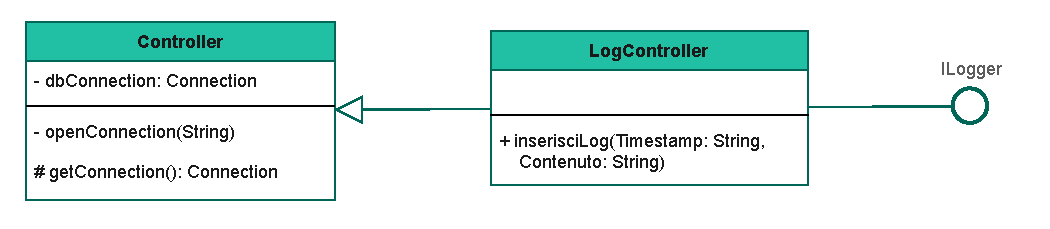
\includegraphics[scale=1]{progettazione/Progettazione-DettagliLog.drawio.pdf}
\end{adjustwidth}
\vspace{0.5cm}

\\
I Controller usano LogController per registrare ogni operazione come Log. A differenza delle altre classi, l'Amministratore può leggere i Log scritti dagli altri controller mediante VisualizzaLog.\\
\vspace{2cm}


\subsection*{Diagramma di Dettaglio: Utente}
\phantomsection
\addcontentsline{toc}{subsection}{Utente}
\vspace{0.5cm}
\begin{adjustwidth}{-1cm}{0cm}
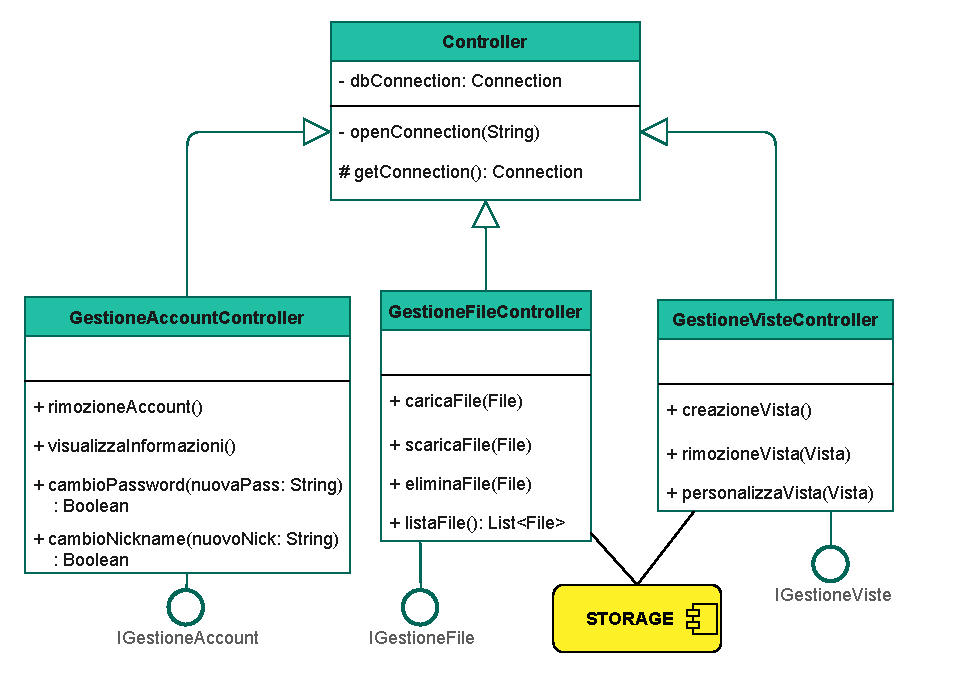
\includegraphics[scale=1]{progettazione/Progettazione-Dettaglio Utente.drawio.pdf}
\end{adjustwidth}
\vspace{0.5cm}

\subsection*{Diagramma di Dettaglio: Gruppi}
\vspace{0.5cm}
\phantomsection
\addcontentsline{toc}{subsection}{Gruppi}
\begin{adjustwidth}{-2cm}{0cm}
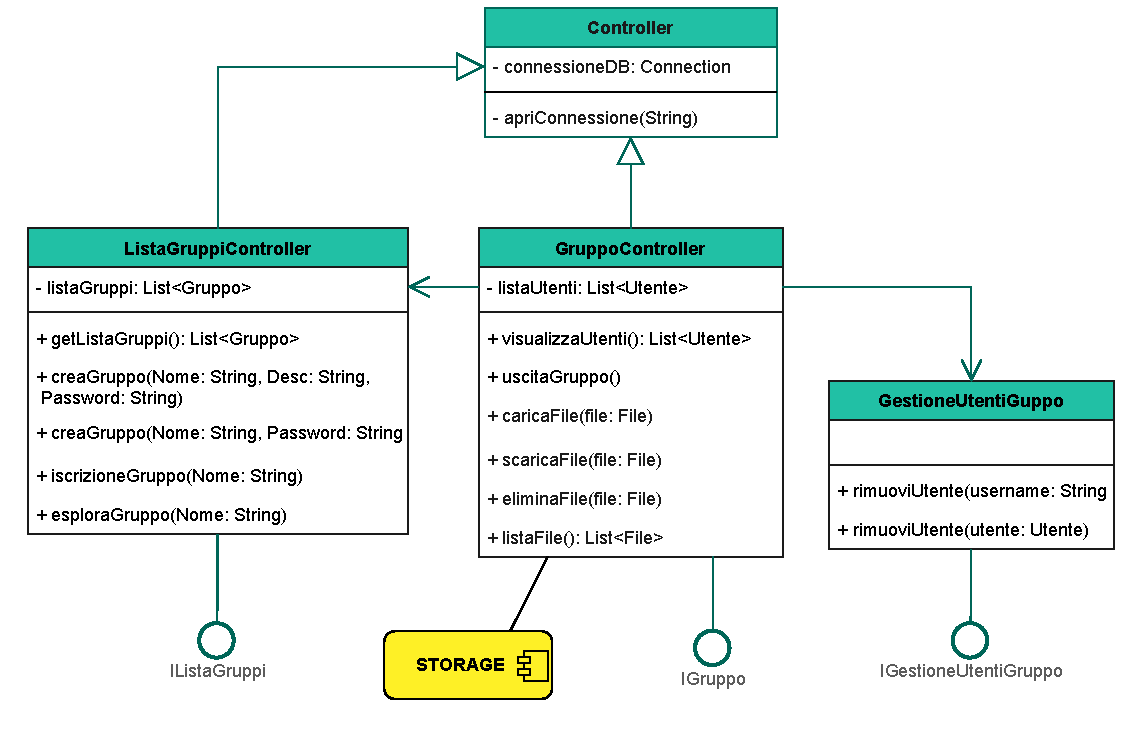
\includegraphics[scale=0.9]{progettazione/Progettazione-DettaglioGruppi.drawio.pdf}
\end{adjustwidth}
\vspace{0.5cm}



\pagebreak
\subsection*{Broker}
\phantomsection
\addcontentsline{toc}{subsection}{Broker}
Nel caso dell' applicazione web, il Broker può essere incorporato nel server web.
\\Così facendo possiamo delegare a quest'ultimo la capacità di gestire le richieste di connessione, catturando le sessioni dei clienti connessi e delegando a sua volta al Controller le operazioni necessarie per eseguire la registrazione e l'autenticazione.\\
Il Broker si interpone tra Client e Server e interagisce fin dalla prima connessione dell'utente al servizio. Potrà inoltre gestire molteplici richieste provenienti da numerosi utenti in parallelo, rendendo l'applicativo accessibile contemporaneamente nelle fasi di autenticazione.
Nel nostro caso specifico, il Broker è incorporato nel framework Dotnet. 
\vspace{0.5cm}



\subsection*{View di Registrazione e Autenticazione}
\phantomsection
\addcontentsline{toc}{subsection}{View di Registrazione e Autenticazione}
\begin{adjustwidth}{-2cm}{0cm}
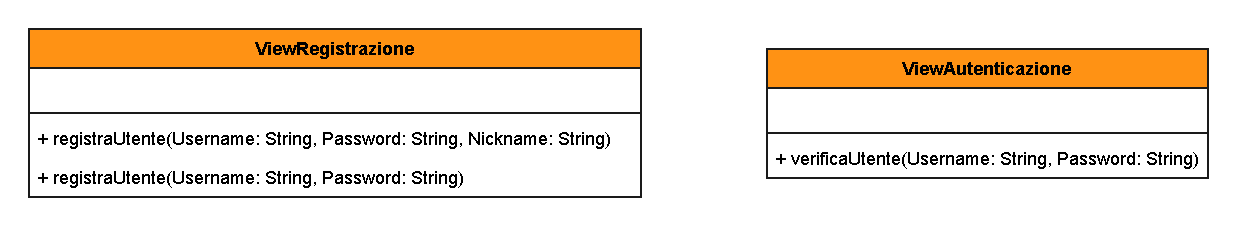
\includegraphics[scale=0.8]{progettazione/Progettazione-Interfacce Disponibili Registrazione_Autenticazione.drawio.pdf}
\end{adjustwidth}
\vspace{0.5cm}
\vspace{0.5cm}




\subsection*{View rese disponibili all' Utente}
\phantomsection
\addcontentsline{toc}{subsection}{View Utente}
\begin{adjustwidth}{-2cm}{0cm}
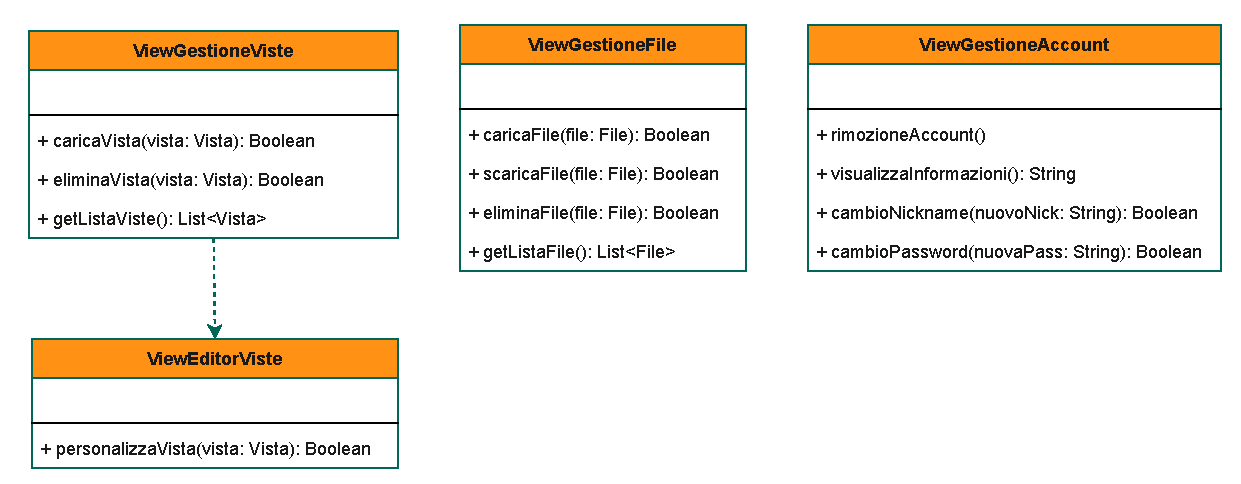
\includegraphics[scale=0.9]{progettazione/Progettazione-Interfacce Disponibili all' Utente.drawio.pdf}
\end{adjustwidth}
\vspace{0.5cm}
\vspace{0.5cm}


\subsection*{View rese disponibili ai Gruppi}
\phantomsection
\addcontentsline{toc}{subsection}{View Amministratore di Gruppo}
\begin{adjustwidth}{-3cm}{0cm}
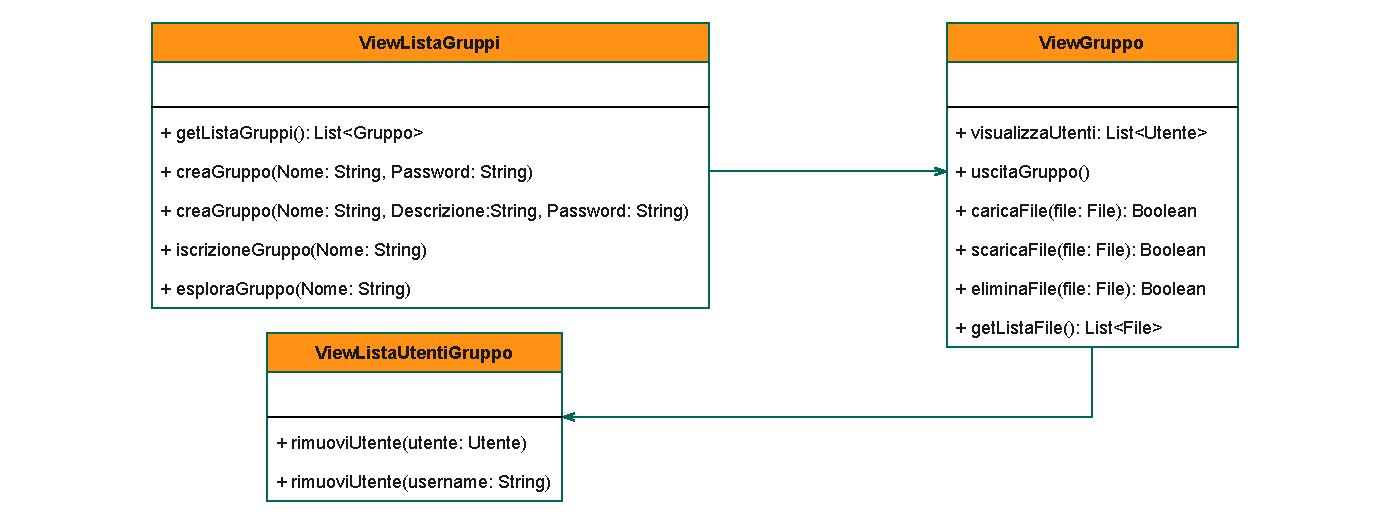
\includegraphics[scale=0.9]{progettazione/Progettazione-Interfacce Disponibili ai Gruppi.drawio.pdf}
\end{adjustwidth}
\vspace{0.5cm}


\subsection*{View rese disponibili all' Amministratore}
\phantomsection
\addcontentsline{toc}{subsection}{View Amministratore}
\begin{adjustwidth}{-2.5cm}{0cm}
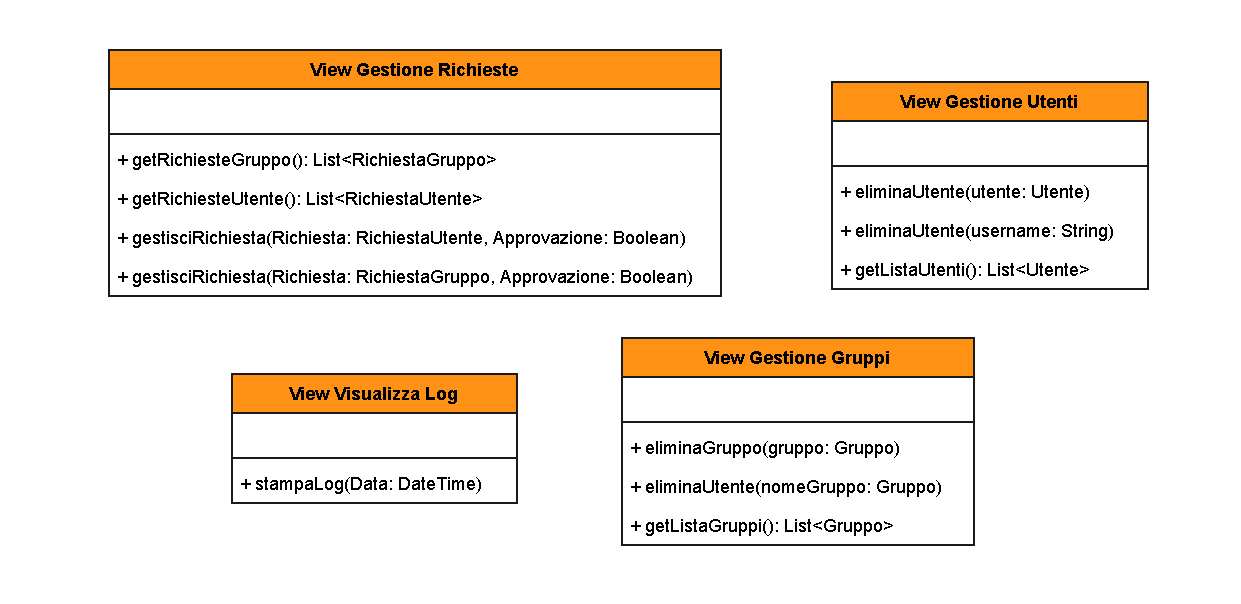
\includegraphics[scale=0.9]{progettazione/Progettazione-Interfacce Disponibili all' Amministratore.drawio.pdf}
\end{adjustwidth}
\vspace{0.5cm}



%----------------------------

\section*{Interfacce Applicazione}
\phantomsection
\addcontentsline{toc}{section}{Interfacce Applicazione}
\vspace{0.5cm}

\subsection*{Autenticazione}
\phantomsection
\addcontentsline{toc}{subsection}{Autenticazione}

\vspace{3cm}

\begin{adjustwidth}{-0.5cm}{0cm}
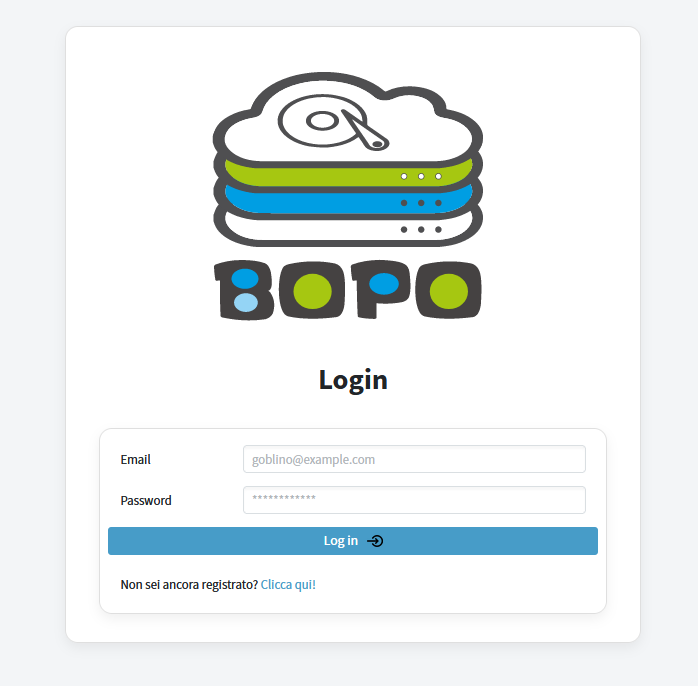
\includegraphics[scale=0.8]{figs/login.png}
\end{adjustwidth}
\pagecolor{background}\afterpage{\nopagecolor}



\subsection*{Registrazione}
\phantomsection
\addcontentsline{toc}{subsection}{Registrazione}
\vspace{3cm}
\begin{adjustwidth}{-0.5cm}{0cm}
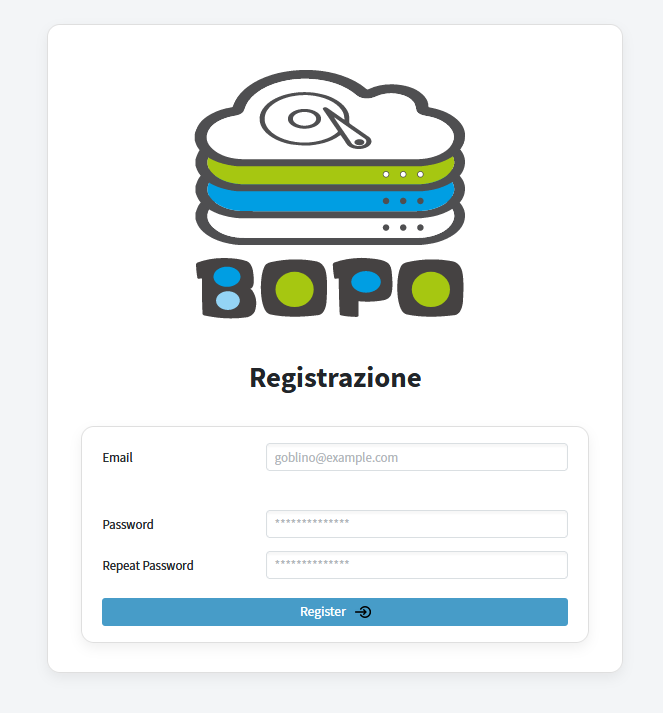
\includegraphics[scale=0.85]{figs/registrazione.png}
\end{adjustwidth}
\pagecolor{background}\afterpage{\nopagecolor}


\subsection*{Gestione Account}
\phantomsection
\addcontentsline{toc}{subsection}{Gestione Account}
\vspace{3cm}
\begin{adjustwidth}{-1.5cm}{0cm}
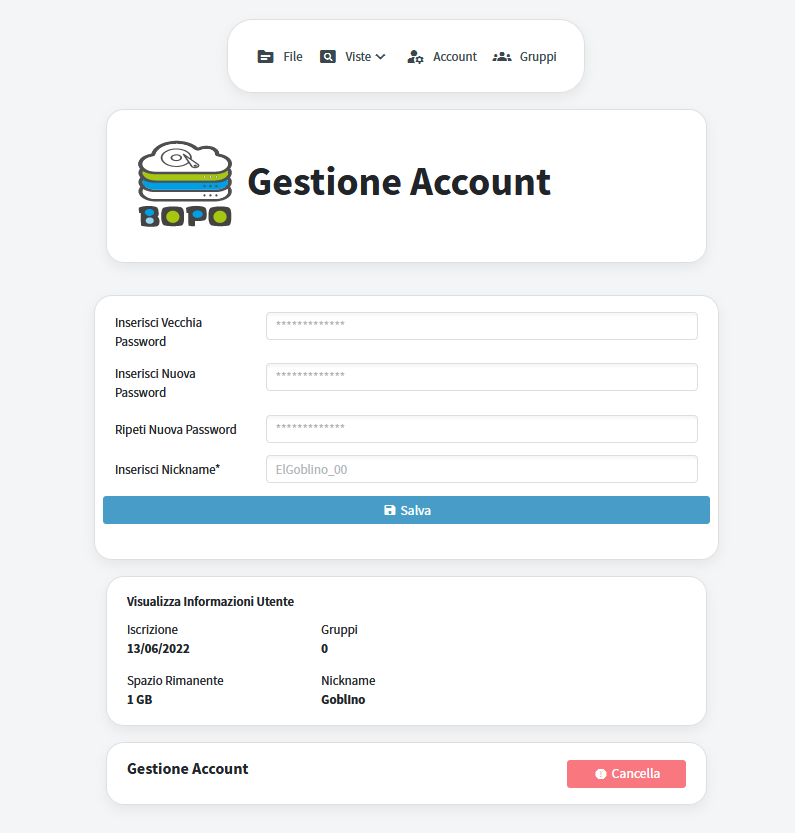
\includegraphics[scale=0.8]{figs/gestione_account.png}
\end{adjustwidth}
\pagecolor{background}\afterpage{\nopagecolor}



\subsection*{Gestione File}
\phantomsection
\addcontentsline{toc}{subsection}{Gestione File}
\vspace{3cm}
\begin{adjustwidth}{-4cm}{0cm}
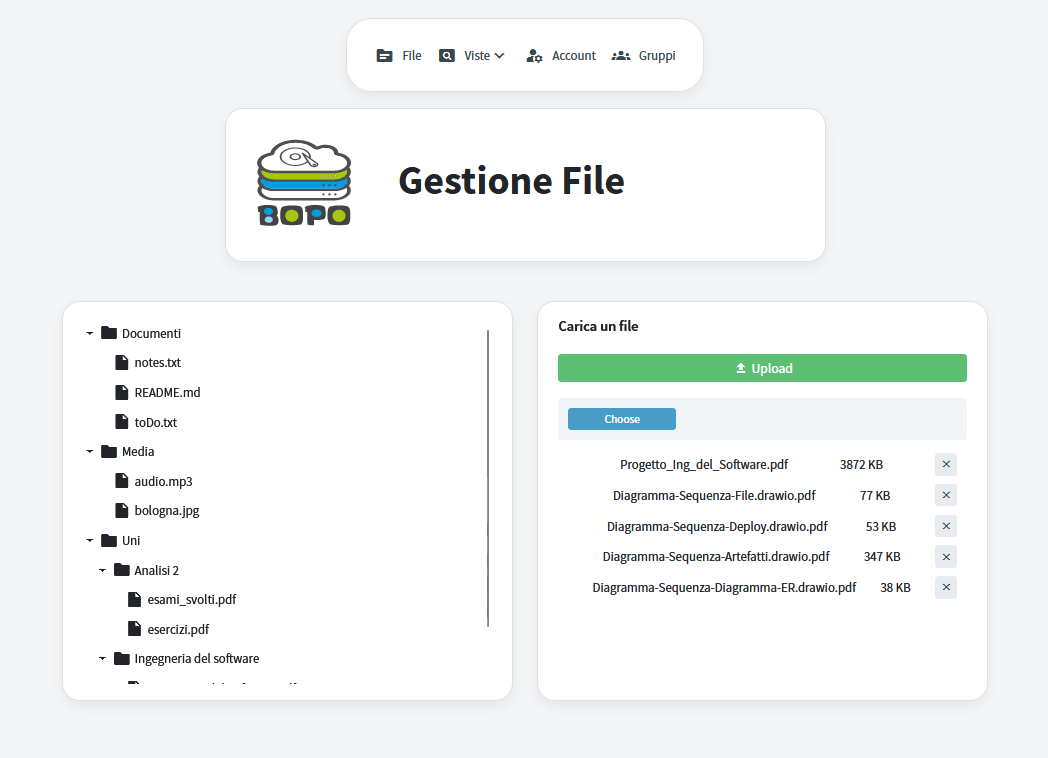
\includegraphics[scale=0.8]{figs/gestione_file.png}
\end{adjustwidth}
\pagecolor{background}\afterpage{\nopagecolor}


\subsection*{Gruppi}
\phantomsection
\addcontentsline{toc}{subsection}{Gruppi}
\vspace{3cm}
\begin{adjustwidth}{-3cm}{0cm}
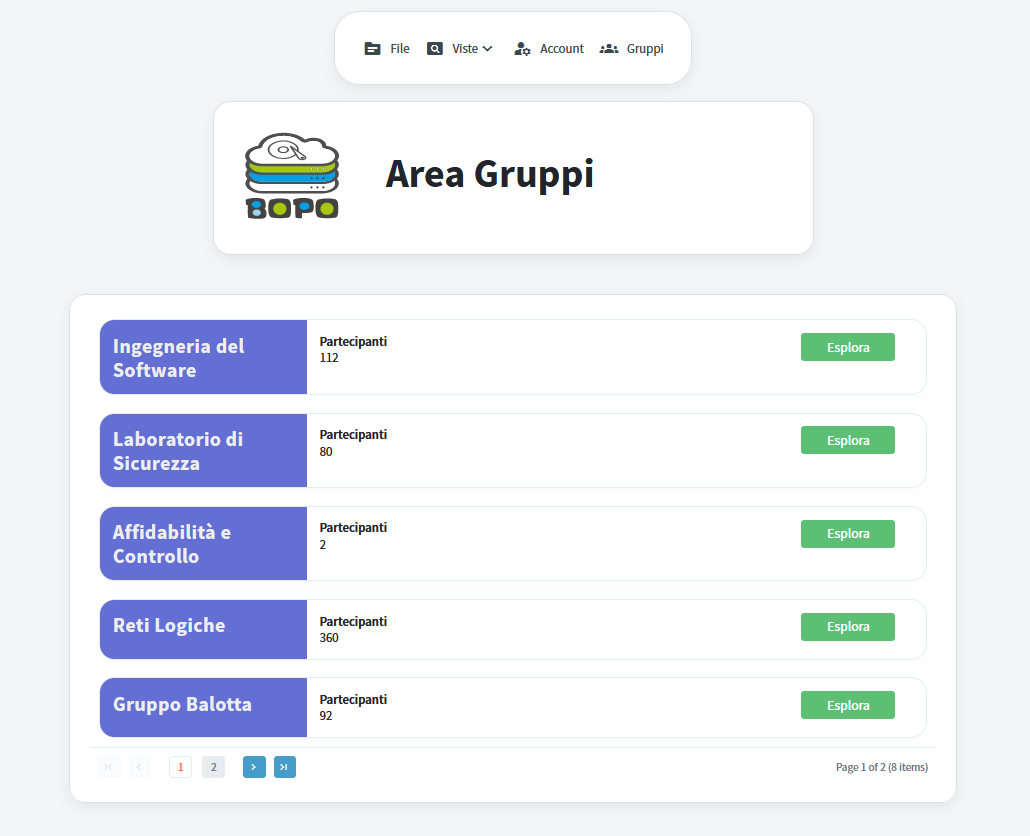
\includegraphics[scale=0.75]{figs/gruppi.png}
\end{adjustwidth}
\pagecolor{background}\afterpage{\nopagecolor}

%--------------------------------






\section*{Diagramma di dettaglio: Interazione}
\phantomsection
\addcontentsline{toc}{section}{Diagramma di dettaglio: Interazione}
\vspace{0.5cm}



\subsection*{Diagramma di Sequenza: Registrazione}
\phantomsection
\addcontentsline{toc}{subsection}{Diagramma di Sequenza: Registrazione}
\vspace{2cm}
\begin{adjustwidth}{-2cm}{0cm}
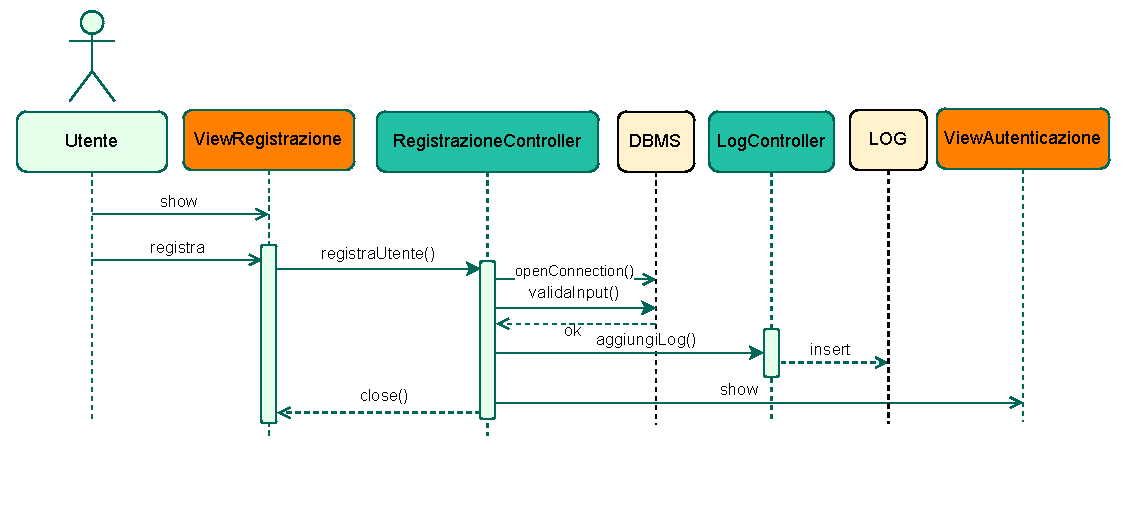
\includegraphics[scale=0.9]{progettazione/Diagramma-Sequenza-Interazione-Registrazione.drawio.pdf}
\end{adjustwidth}
\vspace{0.5cm}
Nella fase di registrazione, l'Utente non interroga direttamente il database. La richiesta deve essere approvata in primo luogo dall' Amministratore, il quale avrà i metodi delegati alla connessione e interrogazione del database dei dati degli Utenti.
Ogni tentativo di autenticazione viene registrato in un altro database che mantiene in modo persistente i Log di sistema.

\subsection*{Diagramma di Sequenza: Autenticazione}
\phantomsection
\addcontentsline{toc}{subsection}{Diagramma di Sequenza: Autenticazione}
\vspace{2cm}
\begin{adjustwidth}{-2cm}{0cm}
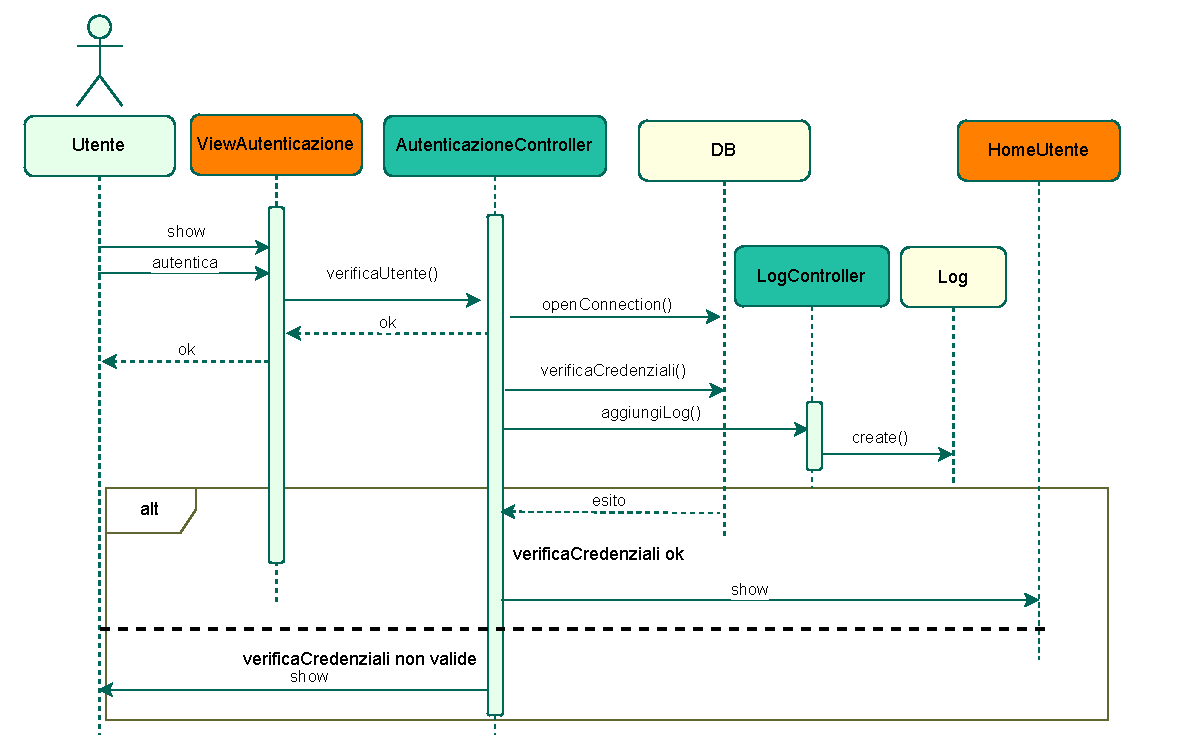
\includegraphics[scale=0.9]{progettazione/Diagramma-Sequenza-Interazione-Autenticazione.drawio.pdf}
\end{adjustwidth}
\vspace{0.5cm}
La fase di autenticazione inserisce i log nel database della persistenza in ogni tentativo di autenticazione. Nel Login si interroga invece il database dei dati degli Utenti.

\subsection*{Diagramma di Sequenza: Gestione Amministratore}
\phantomsection
\addcontentsline{toc}{subsection}{Diagramma di Sequenza: Gestione Amministratore}
\begin{adjustwidth}{-1cm}{0cm}
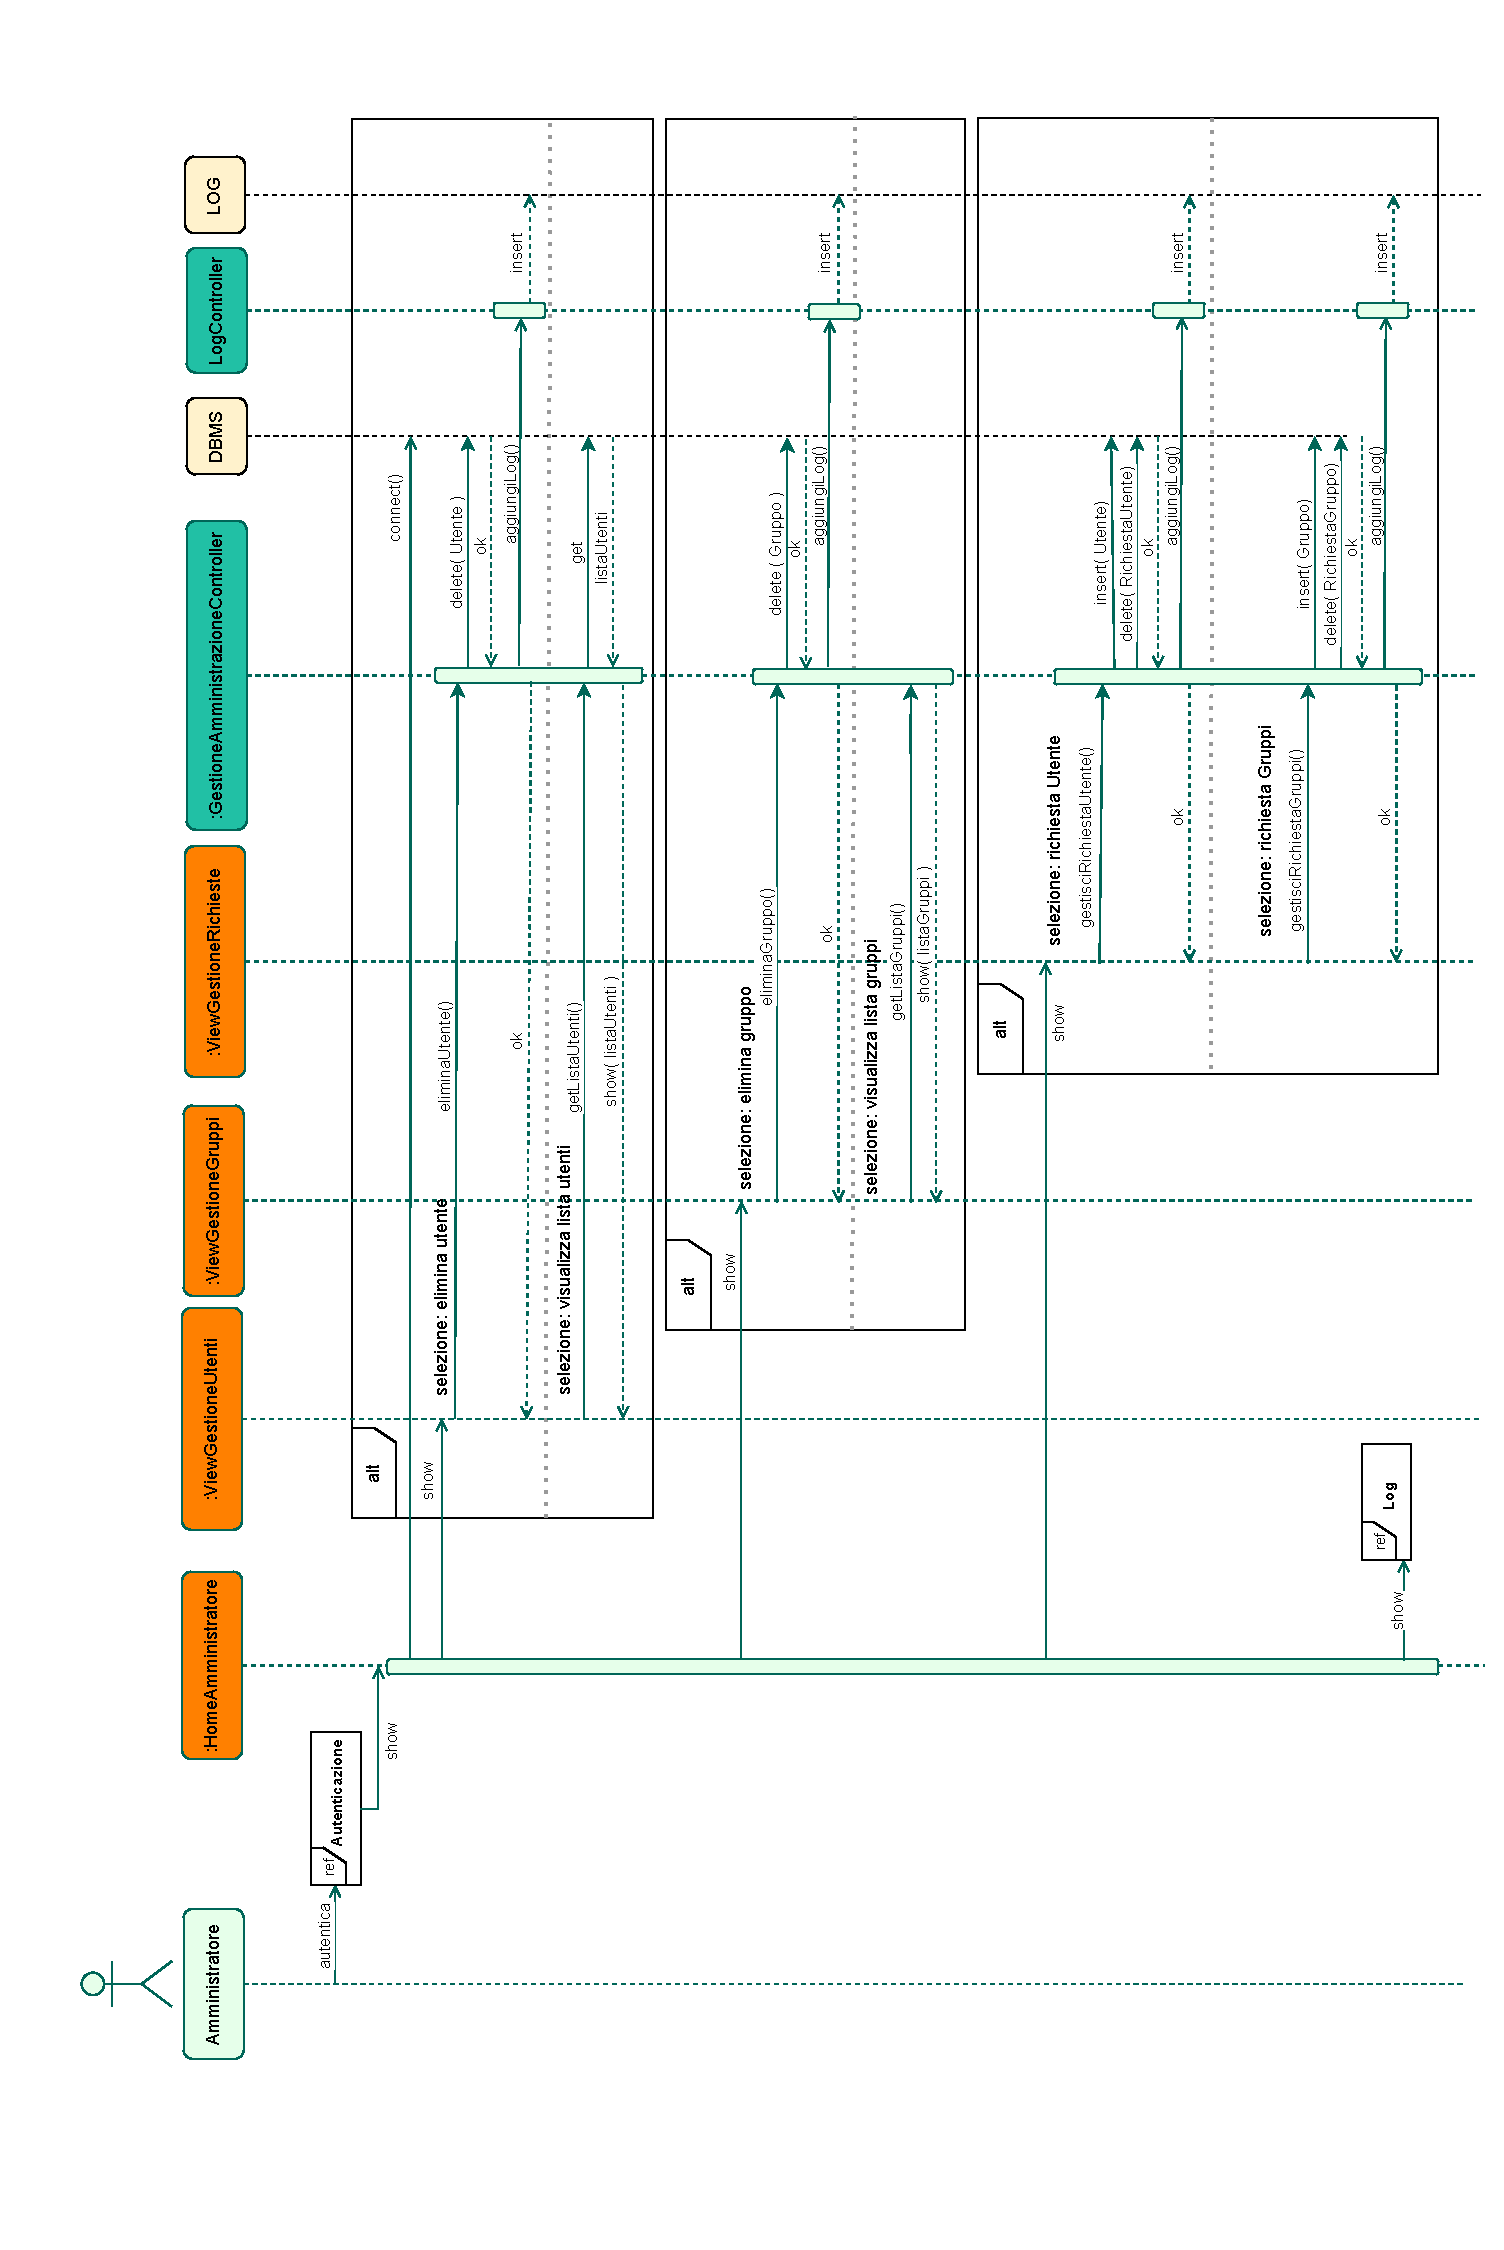
\includegraphics[scale=0.75]{progettazione/Diagramma-Sequenza-Interazione-GestioneAmministratore.drawio.pdf}
\end{adjustwidth}
\vspace{0.5cm}
L'Amministratore ha il ruolo di accettare la coda di richieste provenienti dagli Utenti e dai Gruppi. Si distinguono in questa fase le richieste dell' Utente da quelle del Gruppo. Dopo l'accettazione di una delle due richieste, si raggiungerà lo stesso database Utente/Gruppo in cui verranno registrate le nuove informazioni scatenate dalla richiesta.



\subsection*{Diagramma di Sequenza: Interazione Area Personale\-Viste}
\phantomsection
\addcontentsline{toc}{subsection}{Diagramma di Sequenza: Interazione Area Personale\-Viste}
\begin{adjustwidth}{-2.5cm}{0cm}
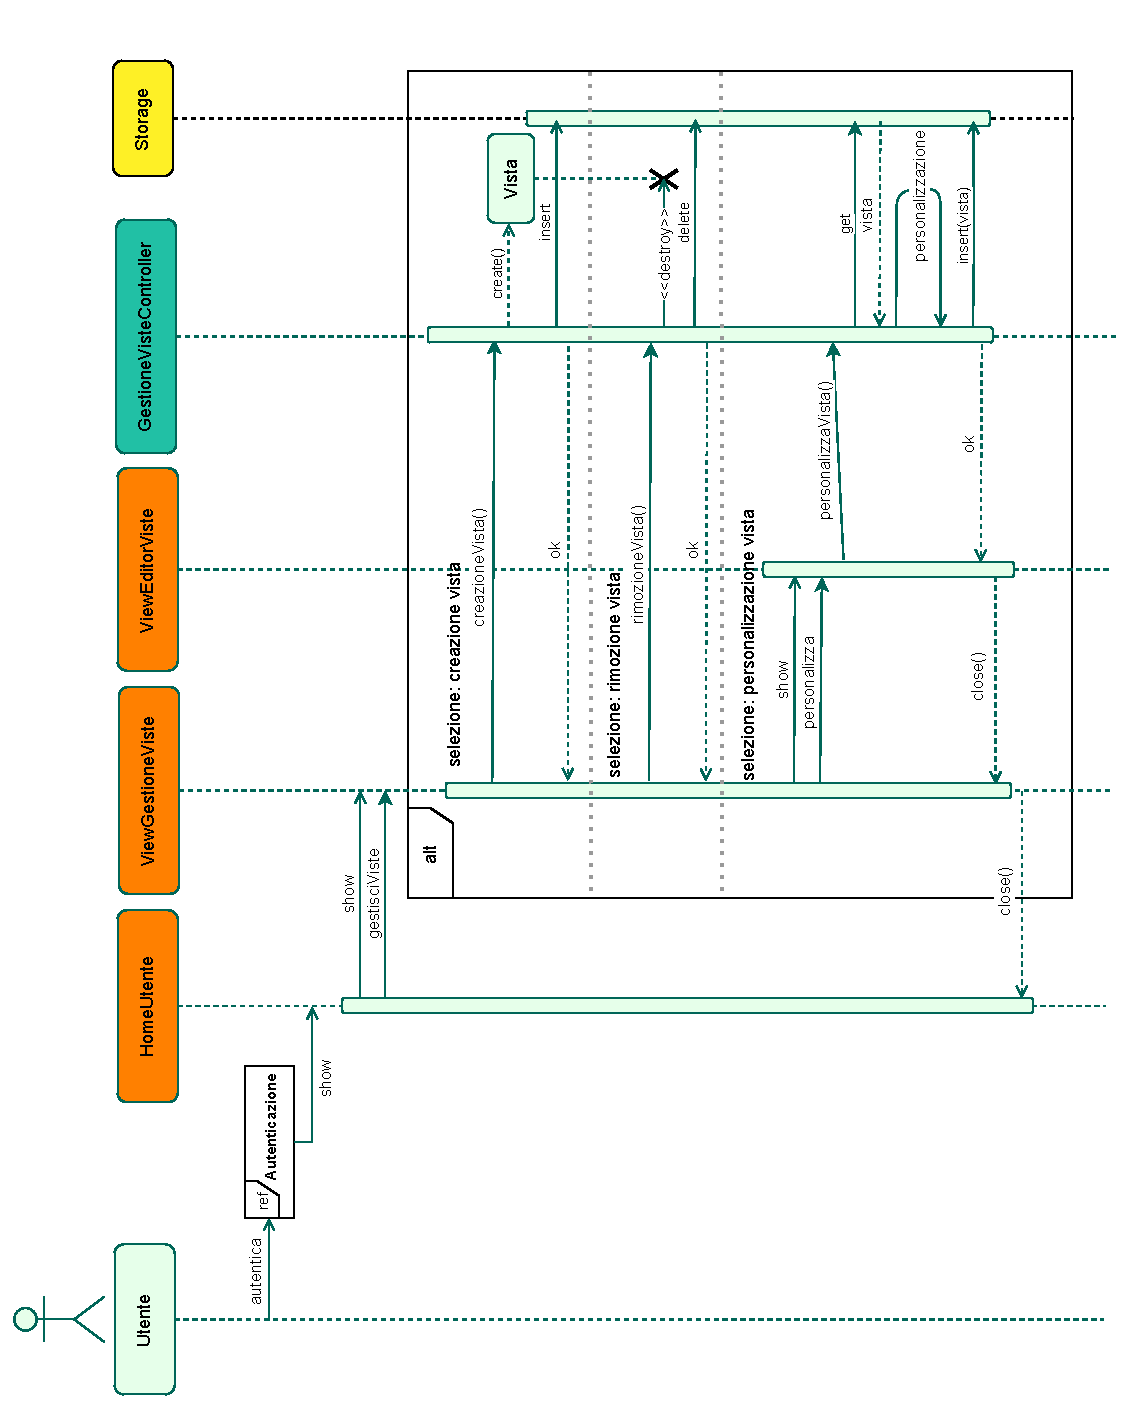
\includegraphics[scale=0.8]{progettazione/Diagramma-Sequenza-Interazione-Viste.drawio.pdf}
\end{adjustwidth}
\vspace{0.5cm}


\subsection*{Diagramma di Sequenza: Interazione Area Gruppi}
\phantomsection
\addcontentsline{toc}{subsection}{Diagramma di Sequenza: Interazione Area Gruppi}
\begin{adjustwidth}{-1.5cm}{0cm}
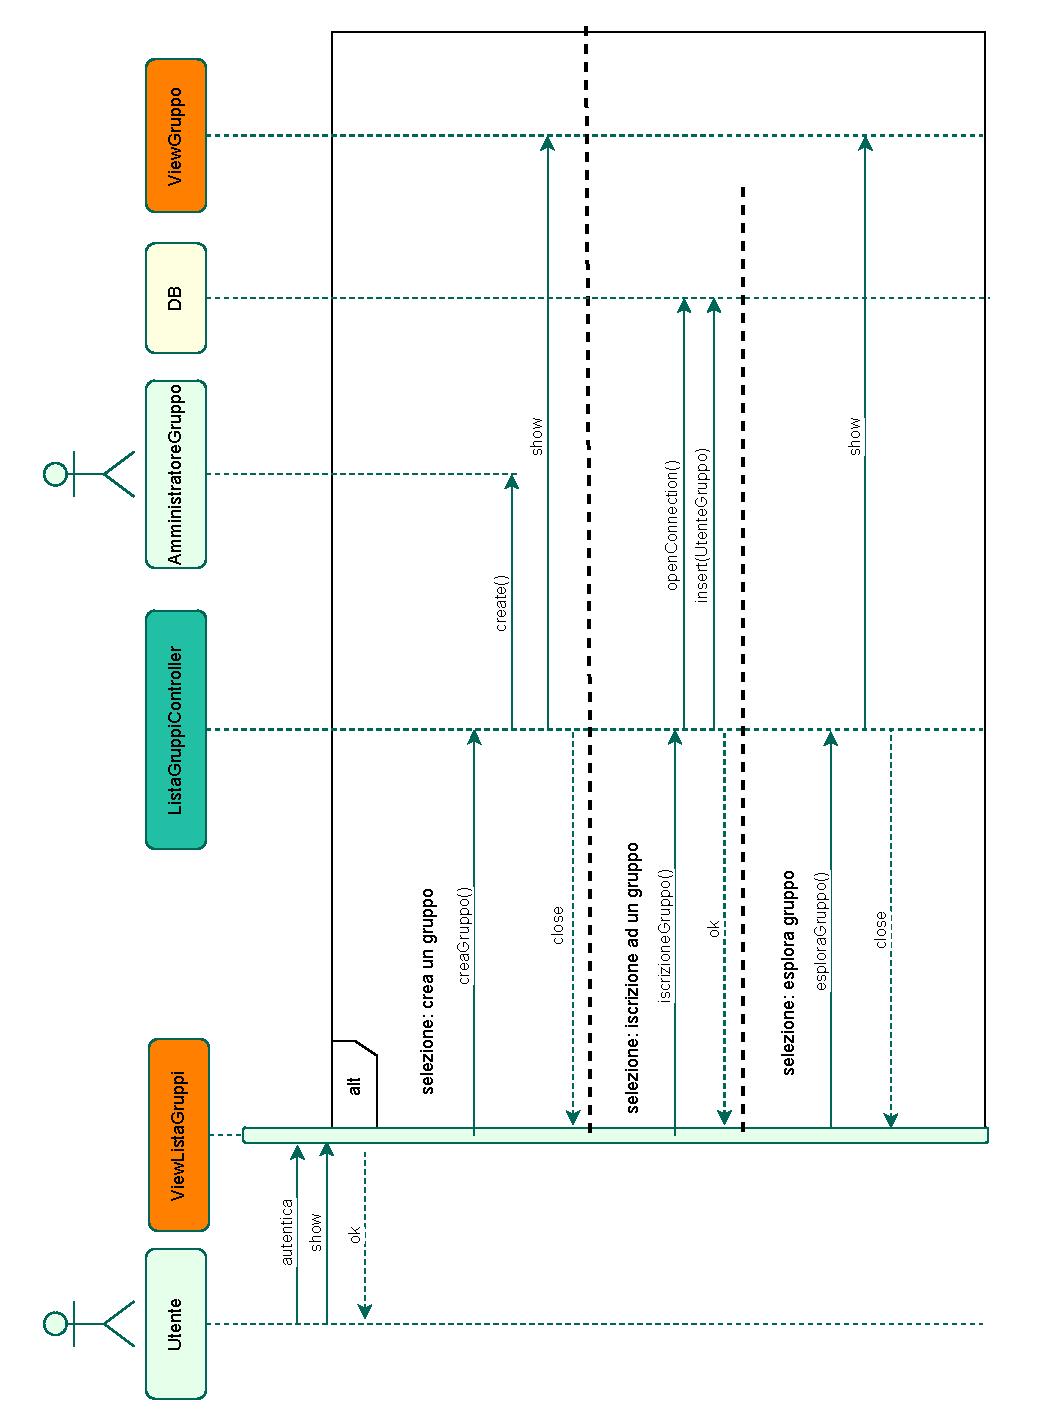
\includegraphics[scale=0.95]{progettazione/Diagramma-Sequenza-Interazione-AreaGruppi.drawio.pdf}
\end{adjustwidth}
\vspace{0.5cm}


\subsection*{Diagramma di Sequenza: Interazione Log}
\phantomsection
\addcontentsline{toc}{subsection}{Diagramma di Sequenza: Interazione Log}
\vspace{1.5cm}
\begin{adjustwidth}{0cm}{0cm}
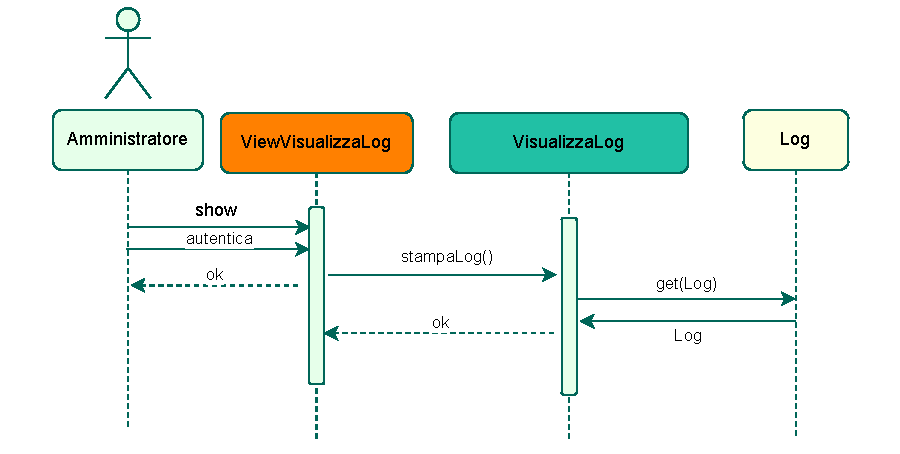
\includegraphics[scale=1]{progettazione/Diagramma-Sequenza-Interazione-Log.drawio.pdf}
\end{adjustwidth}
\vspace{0.5cm}


%---------------------------------------------------------


\pagebreak
\section*{Progettazione Persistenza}
\phantomsection
\addcontentsline{toc}{section}{Progettazione Persistenza}
\vspace{1cm}
La persistenza del \verb|DatabaseUtentiGruppi| verrà implementata utilizzando un DBMS, in particolare MariaDB.
\vspace{0.5cm}
\subsection*{Diagramma Entity-Relation}
\phantomsection
\addcontentsline{toc}{subsection}{Diagramma E-R}
\vspace{0.5cm}
\begin{adjustwidth}{-2cm}{0cm}
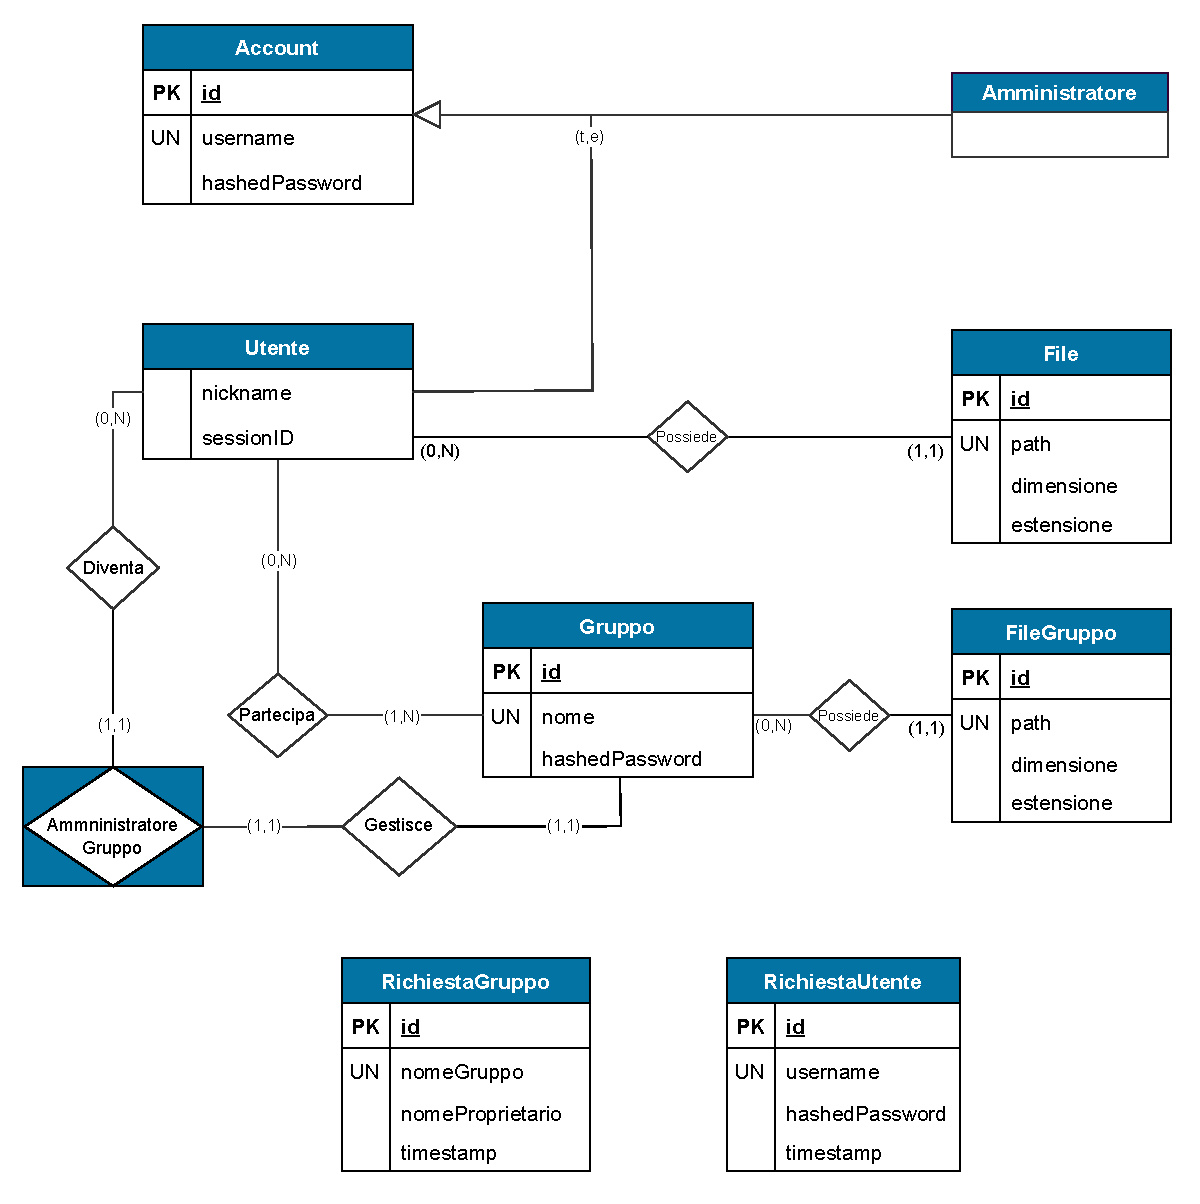
\includegraphics[scale=0.9]{progettazione/Diagramma-Sequenza-Diagramma-ER.drawio.pdf}
\end{adjustwidth}
\vspace{0.5cm}


\vspace{1cm}
\subsection*{Persistenza File}
\phantomsection
\addcontentsline{toc}{subsection}{Persistenza File}
\vspace{0.5cm}
\begin{adjustwidth}{-1cm}{0cm}
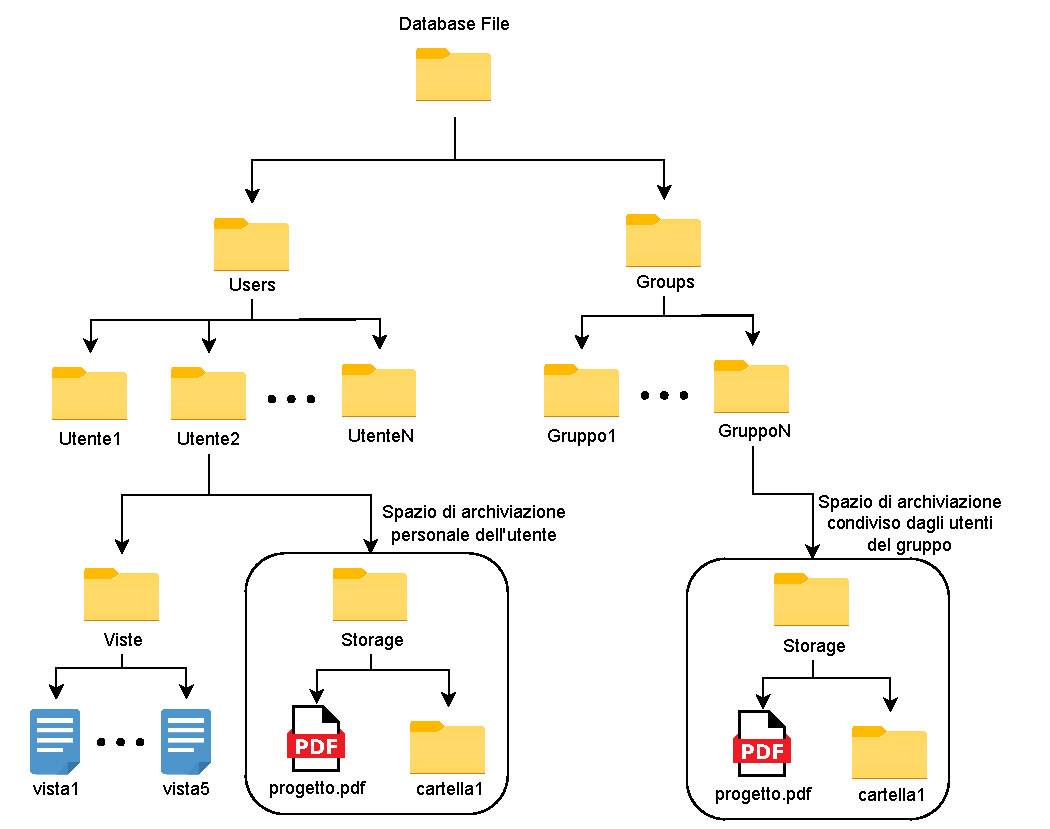
\includegraphics[scale=1]{deployment/Diagramma-Sequenza-File.drawio.pdf}
\end{adjustwidth}
\vspace{0.5cm}

\phantomsection
\addcontentsline{toc}{subsection}{Formato Log}
\vspace{0.5cm}


\subsection*{Formato Log}
I file di Log vengono memorizzati giornalmente attraverso il DatabaseLog. Ogni giorno viene generato un nuovo file così da tener traccia degli accessi al sistema e degli eventi.\\
\\
Ogni entry rispetta questo formato:\\

    \begin{tabular}{|p{3cm} p{3cm} p{3cm}|}
    \hline
    \verb |yyyy-mm-dd-hh-mm| & : \verb|event| & : \verb|data|\\
    \hline
    Timestamp   & Evento che ha generato il Log & Contenuto del Log \\
    \hline
    \end{tabular}
    
    
    
\pagebreak
\section*{Progettazione Collaudo}
\phantomsection
\addcontentsline{toc}{section}{Progettazione Collaudo}
\vspace{1cm}

\inputminted
[
frame=lines,
framesep=2mm,
baselinestretch=1.2,
bgcolor=opal!20!,
fontsize=\footnotesize,
linenos
]
{csharp}{code/collaudo.cs}
%----------------------------------------


\pagebreak
\section*{Deployment}
\phantomsection
\addcontentsline{toc}{section}{Deployment}
\subsection*{Artefatti}
\vspace{1cm}
\phantomsection
\addcontentsline{toc}{subsection}{Artefatti}
\vspace{0.5cm}
\begin{adjustwidth}{0cm}{0cm}
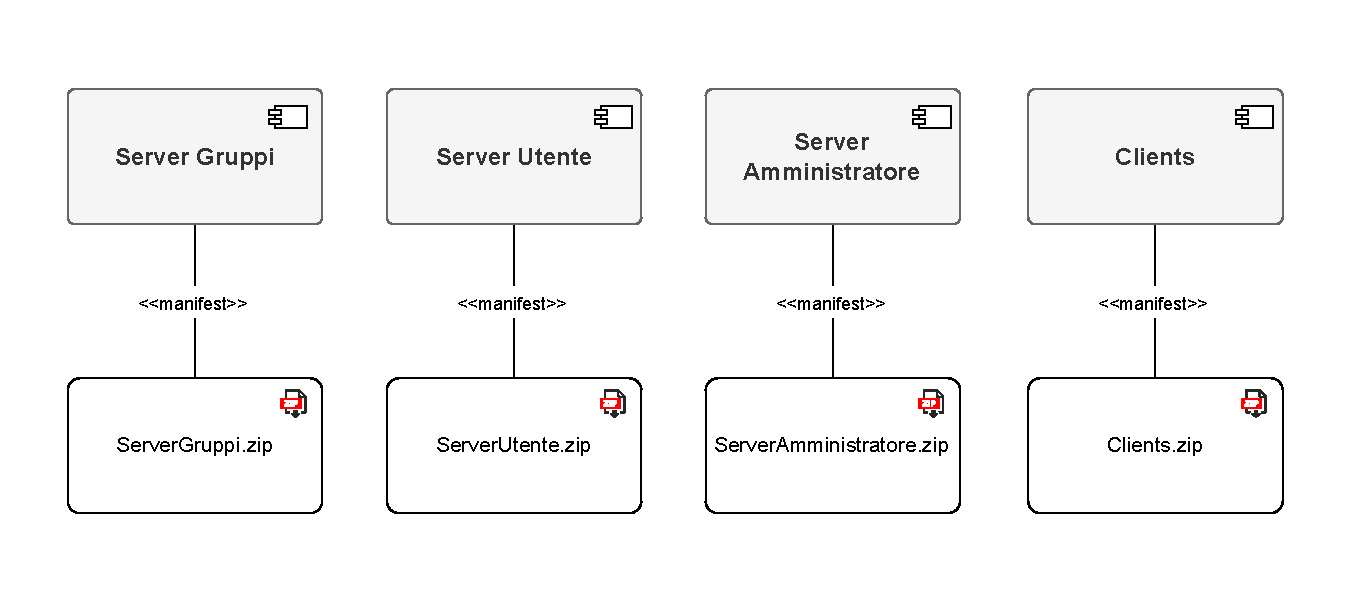
\includegraphics[scale=1]{deployment/Diagramma-Sequenza-Artefatti.drawio.pdf}
\end{adjustwidth}

\vspace{1cm}
\subsection*{Deploy}
\phantomsection
\addcontentsline{toc}{subsection}{Deploy}
\vspace{0.5cm}
\begin{adjustwidth}{-3cm}{0cm}
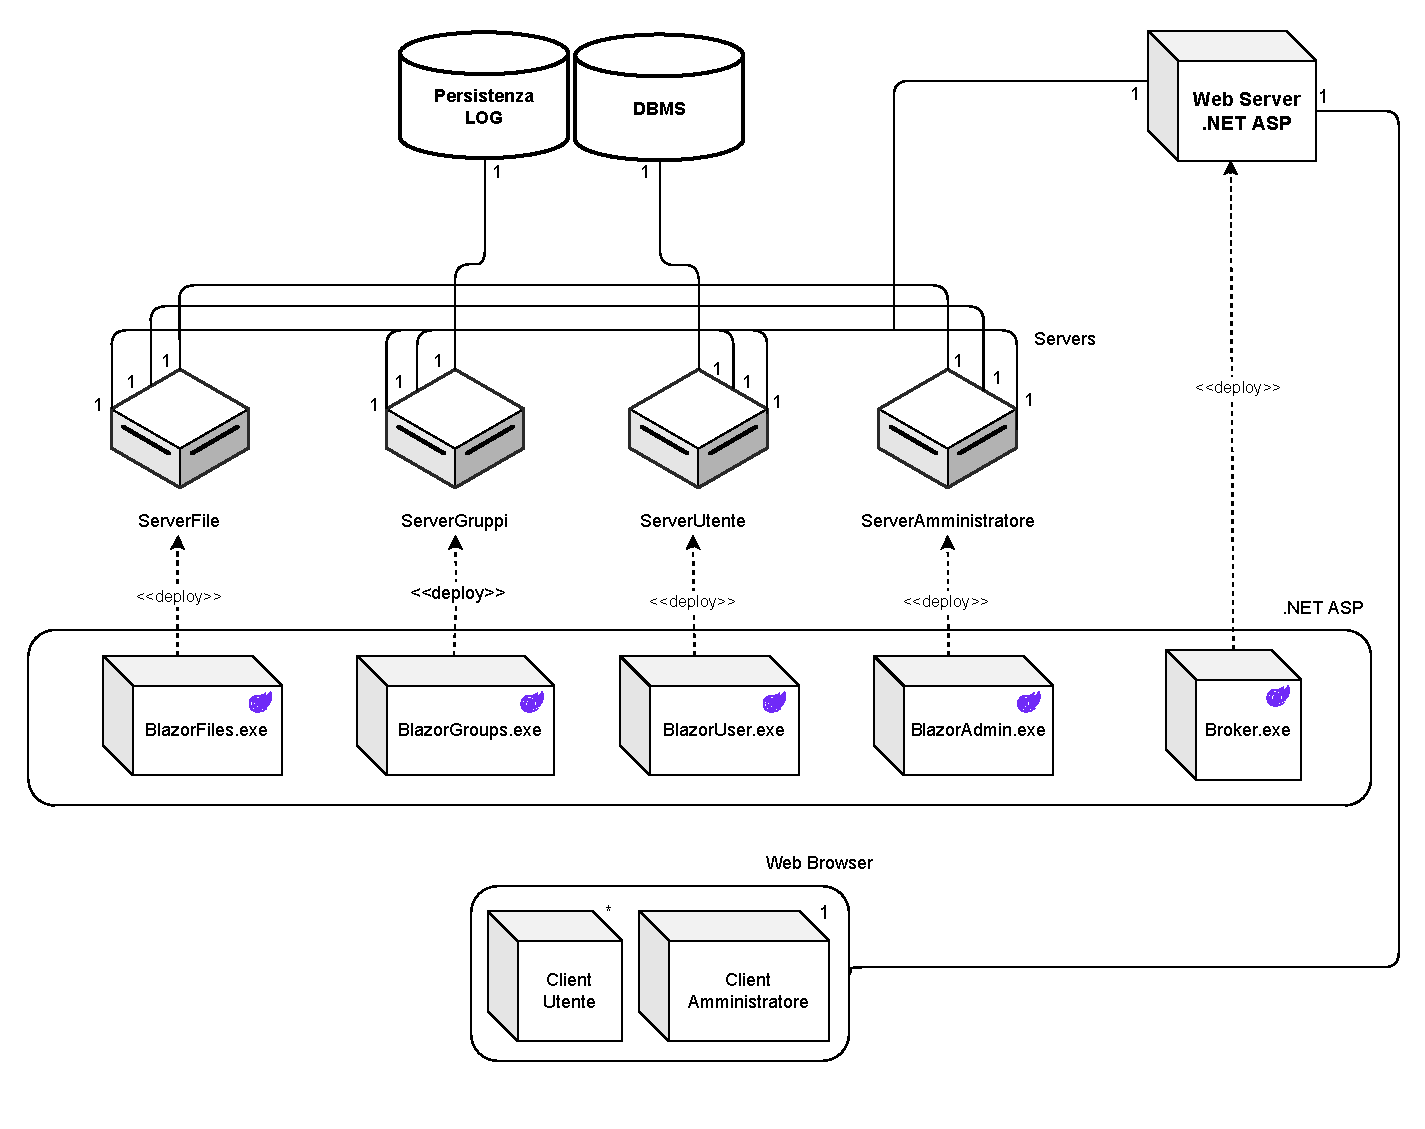
\includegraphics[scale=0.8]{deployment/Diagramma-Sequenza-Deploy.drawio.pdf}
\end{adjustwidth}